\documentclass[oneside]{thesis}
\usepackage{hyperref}
\usepackage{amsfonts}
\usepackage{amsbsy}
\usepackage{amsmath}
\usepackage{amsthm}
\usepackage{amssymb}
\DeclareOldFontCommand{\bf}{\normalfont\bfseries}{\mathbf}
\usepackage[localise,extrafootnotefeatures]{xepersian}
\settextfont[Scale=1]{HM FElmi}
\setdigitfont{Yas}
\settextfont[Scale=1,ExternalLocation=fonts/, BoldFont={HM_FElmiBd}]{HM_FElmi}

\setdigitfont[ExternalLocation=fonts/]{Yas.ttf}

\input{renewdefs.tex}  % My symbols

%\localisecommands
\setcounter{tocdepth}{1} % Dont show sub subsections in ToC.

\begin{document}


\logo{
\includegraphics{logo}}
\date{\vspace{1cm}
	تابستان ۱۳۹۹
}
\title{\LARGE
	جداسازی کور مخلوط‌های غیرخطی فرآیندهای تصادفی
}
\author{بهراد منیری}
\consult{دکتر محمد معماریان}
\university{دانشگاه صنعتی شریف\\دانشکده‌ی مهندسی برق}
\subject{‌}
\supervisor{دکتر مسعود بابائی‌زاده}
\frontmatter
\makethesistitle \pagestyle{empty} \baselineskip1.1\baselineskip

\begin{قدردانی}
از جناب آقای دکتر بابائی‌زاده   که من را با  موضوع بسیار جذاب جداسازی کور منابع آشنا نمودند و با پیشنهاد‌ها و راهنمایی‌های  خود، من را در پیش‌برد این پروژه بسیار یاری کردند، کمال تشکر را دارم. از آقای وفا خلیقی  نیز که با طراحی بسته‌ی \XePersian\ کمک بزرگی به حروف‌چینی فارسی کردند، بسیار سپاس‌گزارم.
\end{قدردانی}

\begin{چکیده}
		{جداسازی کور منابع، فرآیند‌های تصادفی، اطلاعات متقابل، فرآیند‌های گوسی، تحلیل مؤلفه‌های مستقل}
در  این پروژه، ابتدا به تعریف مسئله‌ی جداسازی کور منابع می پردازیم. بعد از مرور قضایای جدایی‌پذیری در مخلوط های خطی، چالش‌های موجود در جداسازی مخلوط‌های غیرخطی را مطرح کرده و نشان می‌دهیم در کلّی‌ترین حالت ممکن، جداسازی کور مخلوط‌های غیرخطی با روش‌های مبتنی بر  استقلال لحظه‌ای منابع (استقلال متغیرهای تصادفی) ممکن نیست و برای این جداسازی، نیاز به وجود شرطی قوی‌تر داریم. با توجه به نتایج تجربی موجود در ادبیات این حوزه، ایده‌ی استفاده از وابستگی‌های زمانی‌ سیگنال‌ها  و جایگزینی استقلال لحظه‌ای منابع  (استقلال متغیرهای تصادفی) با استقلال  کامل منابع (استقلال فرآیندهای تصادفی) را مطرح کرده و تلاش می‌کنیم با بهره بردن از آن، قضیه‌ای عمومی برای جداسازی مخلوط‌های غیرخطی ارائه کنیم و  به بررسی نتایج جدید مبتنی بر این ایده می‌پردازیم. در خلال این کار، به بیان حالاتی خاص از توابع غیرخطی و ناهموار که حتی با وجود فرض استقلال فرآیند‌های تصادفی ورودی (منابع) لزوماً قابل جداسازی نیستند می‌پردازیم.  الگوریتمی بر مبنای کمینه‌سازی اطلاعات متقابل برای جداسازی مخلوط‌های غیرخطی ارائه می‌کنیم و عملکرد آن را در جداسازی مخلوطی خاص مورد بررسی قرار می‌دهیم. در انتها نیز مسئله‌ی جداسازی کور فرآیند‌های تصادفی گوسی را مورد بررسی قرار داده، روش‌های مختلفی برای اجرا این جداسازی ارائه‌ کرده و عملکرد آن‌ها را با هم مقایسه می‌کنیم.
\end{چکیده}

\pagestyle{plain}\pagenumbering{tartibi}\tableofcontents\listoffigures

\mainmatter \pagestyle{headings} \baselineskip1.1\baselineskip
%%%%%%%%%%%%%%%%%%%%%%%%%%%%%%%%%%%%%%%%%%%%%%%%
\paragraphfootnotes %Make paragraphs in line

\chapter{مقدمه}

جداسازی کور منابع\LTRfootnote{Blind Source Separation} 
یا 
تحلیل مؤلفه‌های مستقل\LTRfootnote{Independent Component Analysis}
مسئله‌ای  در پردازش سیگنال و یادگیری ماشین است که در اویل دهه‌ی ۸۰ میلادی توسط کریستین جوتن\LTRfootnote{Christian Jutten}  مطرح شد
\cite{historicalnotes}. 
در مسئله‌ی جداسازی کور، سیگنال‌های چند منبع مستقل، پس از گذر از یک سیستم با هم مخلوط می‌شوند و این مخلوط‌ها توسط چند گیرنده دریافت می‌گردند. هدف، یافتن منابع اولیه از روی مخلوط‌های آن‌ها و بدون داشتن هیچ اطلاعات اولیه‌ای در مورد منابع یا سیستم مخلوط کننده است. به عنوان مثال،  فرض کنید $n$ نفر در یک اتاق به طور هم‌زمان در حال صحبت هستند.  صحبت این افراد توسط $n$ میکروفن در مکان‌های دلخواهی از این اتاق ذخیره شده است. هدف، جداسازی سیگنال صحبت هر فرد، تنها با مشاهده‌ی سیگنال ذخیره‌شده توسط این میکروفن‌ها، که هر یک مخلوطی از سیگنال صحبت افراد مختلف است، می‌باشد. جداسازی کور منابع می‌تواند در مسائل گوناگون، از جمله جداسازی سیگنال منابع مختلف مغزی در هنگام مطالعه بر روی سیگنال‌های الکتروانسفالوگرام، حذف سایه‌ی پشت یک برگه در هنگام اسکن کردن آن و همچنین مسئله‌ی استنتاج علّی کاربرد داشته باشد.


فرض کنید که  فرآیند‌های تصادفی‌ مستقل
$\s(t) = [s_1(t), s_2(t) \dots, s_n(t)]^\top$،
منابع ما بوده که مشاهده نشده‌اند و فرآیند‌های تصادفی 
$\x(t) = [x_1(t), x_2(t) \dots, x_n(t)]^\top$
مشاهدات ما باشند.   تابع 
$f: \R^n \to \R^n$
تابع مخلوط کننده است و داریم 
$\x(t) = f\Big(\s(t)\Big)$.
در تمام طول این پروژه، فرض شده است که تعداد منابع و مشاهدات برابر $n$ هستند. هدف اصلی مسئله‌ی جداسازی کور منابع، یافتن تابع $f$ و همچنین سیگنال‌های 
$\s(t)$
بر اساس مشاهدات ما از سیگنال‌های 
$\x(t)$
است. این مسئله در حالتی که $f$ یک تابع خطی باشد، به طور کامل حل شده است و شرایط کافی بر روی منابع تا آن‌ها قابل جداسازی باشند به دست آمده است
\cite{ICAbook}.
در حالت غیرخطی، مسئله بسیار دشوارتر است.  در صورتی که فرآیند‌های تصادفی
$\s(t)$
در زمان، وابستگی نداشته باشند، یعنی سفید باشند، می‌توان مثال‌‌های فراوانی از توابع $f$ یافت که این فرآیند‌های مستقل  (که در زمان نیز رابطه‌ای ندارند و 
سفید هستند) را، به فرآیند‌های مستقل تبدیل کند. تا مدت‌ها تصوّر بر این بوده است که اعمال شرط هموار بودن بر تابع 
$f$
جواب این مسئله را یکتا می‌کند، اما در سال 2002، دکتر بابائی زاده مثالی از تابعی هموار ارائه‌ دادند که قادر بود فرآیند‌های سفید مستقل را به فرآیند‌های سفید مستقل تبدیل کند، در حالی که آن‌ها با همدیگر مخلوط ‌شده‌اند. این مثال نشان می‌دهد که در حالتی که فرآیند‌های تصادفی سفید هستند، جداسازی کور منابع غیرخطی مبتنی بر استقلال منابع ممکن نیست
\cite{mbzadehthesis}.
در سال ۲۰۰۳، در
\cite{harmeling2003kernel}
ایده‌ی استفاده از وابستگی‌های زمانی را برای جداسازی ترکیب‌های غیرخطی فرآیند‌های تصادفی مطرح شد. در این مقاله‌ الگوریتمی برای جداسازی ترکیب‌های غیرخطی، با استفاده از روابط زمانی ارائه شده است که علی‌رغم عملکرد تجربی بسیار امیدوارکننده‌ی آن،  تا کنون اثباتی برای صحت عملکرد آن ارائه نشده‌است.  در سال‌های ۲۰۱۶، ۲۰۱۷ و ۲۰۱۹، تلاش‌های مجددی برای اثبات یک قضیه‌ی جدایی‌پذیری انجام گرفت و  دو ایده‌ی یادگیری بر مبنای جایگشت منابع\LTRfootnote{Permutation Contrastive Learning (PCL)}
و یادگیری بر مبنای تمایز بین زمان‌ها\LTRfootnote{Time Contrastive Learning (TCL)} 
مطرح شد
\cite{TCL, PCL, newHyva}.
در این مقالات، قضیه‌هایی جدید برای جدایی‌پذیری ترکیب‌های غیرخطی فرآیند‌های تصادفی ارائه‌ شده‌است. این قضایا، شرایطی بسیار سخت‌گیرانه بر روی فرآیند‌های تصادفی قرار می‌دهد و تا کنون مشخص نیست که این شرایط، تا چه اندازه می‌توانند محدود‌کننده باشند. یکی از اهداف این پروژه، یافتن دسته‌ای از فرآیند‌های تصادفی با شرایط فوق و بررسی میزان محدودیت اعمال شده توسط آن شرایط است. دسته‌ای از ایده‌ها به دنبال یافتن نگاشتی  هستند که تحت آن‌ها، مسئله‌ی جداسازی کور منابع غیرخطی به یک مسئله‌ی خطی تبدیل شود. مقاله‌ی 
\cite{ehsandoust}
یکی از این مقالات است و الگوریتمی ارائه می‌کند که مشتق فرآیند‌های تصادفی منبع را جداسازی می‌کند، اما قادر به اثبات قضیه‌ی جدایی‌پذیری نیست. 

در این رساله، به بررسی مسئله‌ی جداسازی کور مخلوط‌های غیرخطی منابع پرداخته و تلاش می‌کنیم درک بهتری از مسئله پیدا کنیم. در فصل 
\ref{probdef}
مسئله‌ی جداسازی کور مخلوط‌های خطی و  غیرخطی را تعریف  و مثال‌های جدایی‌پذیر را بررسی می‌کنیم و ایده‌ی استفاده از روابط زمانی را مطرح می‌نماییم. فصل 
\ref{chapter:NCE}
به مرور تخمین مبتنی بر تفکیک نویز می‌پردازد. این چارچوب آماری در فصل‌های بعدی برای حل مسئله‌ی جدسازی کور مورد بررسی قرار می‌گیرد.  در فصل 
\ref{seprability}
قضایای جدایی‌پذیری موجود را در حالت غیرخطی بررسی می‌کنیم. در  فصل
\ref{algs}
مروری بر روش‌های کمینه‌سازی اطلاعات متقابل خواهیم داشت و الگوریتمی برای جداسازی مخلوط‌های غیرخطی ارائه کرده و کیفیت عملکرد آن را می‌سنجیم.  در آخر نیز، در فصل
\ref{chapter:gaussian}
بررسی تئوریک و معرفی الگوریتم‌هایی برای جداسازی مخلوط‌های غیرخطی فرآیندهای تصادفی گوسی می‌پردازیم.
\chapter{معرفی مسئله}
\label{probdef}
در این فصل، به تعریف مسئله‌ی جداسازی کور منابع می‌پردازیم و نتایج ابتدایی در این حوزه را مرور می‌کنیم.

\section{جداسازی کور مخلوط‌های خطی}
فرض کنید 
$\s = [s_1, s_2, \dots, s_n]^\top$
بردار منابع باشد که در آن متغیر‌های تصادفی 
$s_i$
مستقل هستند. ماتریس
$A \in \R^{n\times n}$
ماتریسی وارون پذیر باشد که هیچ اطلاعاتی در مورد آن در اختیار نداریم. به این ماتریس، ماتریس مخلوط‌کننده می‌گوییم. $n$ سیگنال 
$\x = [x_1, x_2, \dots, x_n]^\top$
مشاهده شده‌اند که برای آن‌ها داریم:
\begin{equation}
\x = A\s \implies 
\begin{bmatrix}
x_1\\x_2\\\vdots\\x_n
\end{bmatrix} = 
A
\begin{bmatrix}
s_1\\s_2\\\vdots\\s_n
\end{bmatrix}
\end{equation}
هدف ما به دست آوردن بردار 
$\s$
با مشاهده‌ی بردار
$\x$
است. 

برای مثال فرض کنید دو متغیر‌ تصادفی
$s_1$
و 
$s_2$
دو متغیر تصادفی با توزیع
$U[0, 1]$
و مستقل باشند. نمودار پراکنش یک نمونه‌ی دوبعدی از این مسئله‌ را در شکل
\eqref{2dlinear}
دیده می‌شود. یک ایده‌ برای جداسازی این متغیرها یافتن نگاشتی است که شکل سمت راست را به یک مربع نگاشته نماید. در ادامه به بررسی قضایای کلّی جدایی‌پذیری خواهیم پرداخت.

\begin{figure}
	\centering
	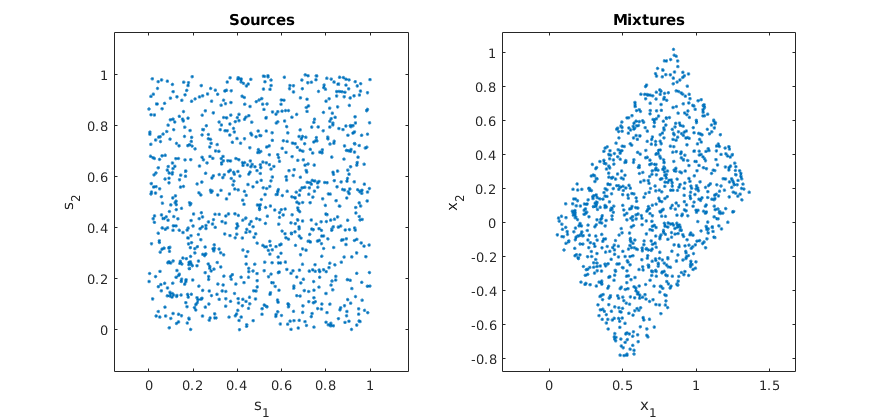
\includegraphics[scale=0.6]{Figures/2dlinear.png}
	\caption{مثالی از ورودی و خروجی یک سیستم مخلوط کننده‌ی خطی دو بعدی}
	\label{2dlinear}
\end{figure}


قضیه‌ی زیر برای اولین بار در
\cite{darmois}
و
\cite{skitovich}
ارائه شده است و از اولین نتایج در جداسازی کور منابع است. 
\begin{theorem}
	\label{darmois_skitovic}
	فرض کنید 
	$X_1,X_2, \dots, X_n$
	متغیرهای تصادفی مستقل باشند. متغیر‌های تصادفی 
	$Y_1,Y_2$
	ر ا به شکل زیر تعریف کنید:
	\begin{equation}
	\begin{cases}
	Y_1 = a_1X_1 + a_2 X_2 + \dots a_NX_N\\
	Y_2 = b_1X_1 + b_2 X_2 + \dots b_NX_N
	\end{cases}
	\end{equation}
	اگر 
	$Y_1$
	و 
	$Y_2$
	مستقل باشند، تمام $X_k$ هایی که برای آن‌ها
	$a_kb_k \neq 0$
	است، گوسی هستند.
\end{theorem}
\begin{proof}
	برای یافتن اثباتی امروز از این قضیه، می‌توانید به 
	\cite{newdarmois}
	مراجعه کنید.
\end{proof}
این قضیه نشان می‌دهد که منابع غیرگوسی مستقل را نمی‌توان به نحوی به صورت خطی مخلوط کرد و متغیر های مستقل در خروجی داشت. در نتیجه  اگر 
$B$
ماتریس جداسازی ما باشد،
سیستم مخلوط‌کننده-جداساز ما
$\y = B\x = BA\x$،
خود یک سیستم خطی است، با فرض غیرگوسی بودن 
$s_i$
ها، مستقل بودن 
$y_i$
ها، جداشدن منابع را تضمین می‌کند. اما در این‌جا چند ابهام وجود دارد، ابهام اول، $y_i$ ها می‌توانند در یک ضریب با منابع متفاوت باشند، زیرا ضرب درایه‌ به درایه‌ی خروجی‌های $y_i$، در استقلال آن‌ها تاثیری ندارد. دوم اینکه، $y_i$ لزوماً مساوی یک ضریب از 
$s_i$
نیست و ممکن است یک جایگشت نیز اتفاق افتاده باشد، زیرا جایگشت نیزاستقلال 
$y_i$
ها را تحت‌الشعاع قرار نمی‌دهد. به طور خلاصه، داریم
$s_i = a_i y_{\sigma(i)}$
که 
$\sigma$
یک جایگشت است و 
$a_i$
ضرایب ثابت هستند.

\section{جداسازی کور مخلوط‌های غیرخطی}

مجدداً فرض کنید $\s = [s_1, s_2, \dots, s_n]^\top$ بردار منابع ما بوده که از آن‌ها اطلاعی نداریم و بردار‌های 
$\x = [x_1, x_2, \dots, x_n]^\top$
مشاهده شده باشند به نحوی که 
$\x = f\big(\s\big)$،
که در آن 
$f : \R^n \to \R^n$
تابع نامعلوم مخلوط‌کننده است. هدف اساسی جداسازی کور منابع غیر خطی، یافتن تابع 
$g : \R^n \to \R^n$
است، به نحوی که اگر تعریف کنیم
$\y = g\big(\x\big) = gof \big(\s\big)$،
داشته باشیم
$y_i = h_i \big(s_{\sigma(i)}\big)$
که در آن 
$\sigma$
یک جایگشت و $h_i$ یک تابع وارون‌پذیر است. توابع‌
$h_i$
دوگان ضرایب 
$a_i$
در جداسازی کور منابع خطی بوده و به این دلیل اضافه شده‌اند که اگر دو متغیر تصادفی مستقل باشند، هر تابع از آن‌ها نیز مستقل خواهد بود. 
$\sigma$
نیز دقیقاً مشابه حالت خطی، بیانگر ابهام در جایگشت است. شکل 
\eqref{nonlinBSS}
مدل جداسازی کور غیرخطی را نشان می‌دهد.

\begin{figure}
	\centering
	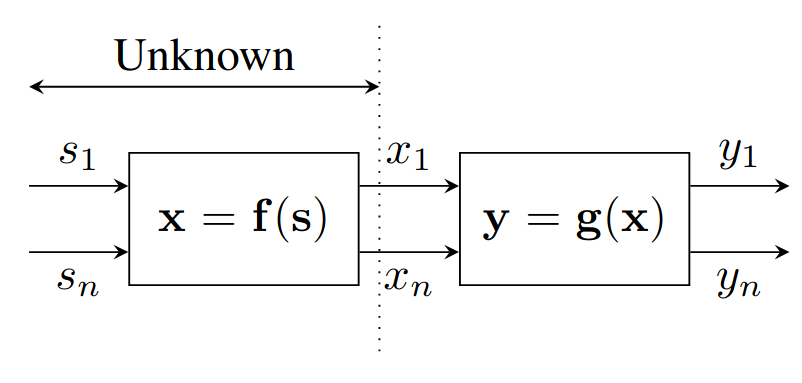
\includegraphics[scale=0.3]{Figures/BSS.png}
	\caption{مدل مسئله‌ی جداسازی کور منابع غیرخطی}
	\label{nonlinBSS}
\end{figure}




مسئله‌ی مهمی که در این‌جا مطرح می‌شود این است که آیا می‌توان قضیه‌ای مشابه قضیه‌ی
\eqref{darmois_skitovic}
برای حالت غیرخطی داشت که تضمین کند اگر یک تابع 
$g$
قادر باشد مشاهدات را به متغیر‌های تصادفی مستقلی نگاشت کند، آن‌ها را جدا کرده است یا خیر. این گزاره در حالت کلی درست نیست. در ادامه به بررسی یک مثال نقض خواهیم پرداخت.
\begin{example}
	فرض  کنید 
	$s_1$
	یک متغیر تصادفی رایلی با توزیع
	$p_{s_1}(s_1) = s_1 \exp (\s_1^2/2)$
	باشد. 
	$s_2$
	را نیز یک متغیر تصادفی یکنواخت در بازه‌ی 
	$[0, 2\pi)$
	در نظر بگیرید که از 
	$s_1$
	مستقل است. در این حالت، مخلوط زیر را بررسی می‌کنیم:
	\begin{equation}
	\begin{cases}
	y_1 = s_1 \cos(s_2)\\
	y_2 = s_1 \sin(s_2)
	\end{cases}
	\end{equation}
	ژاکوبین این تبدیل برابر است با:
	\begin{equation}
	\mathbf{J}(s_1, s_2) = 
	\begin{bmatrix}
	\cos(s_2) & -s_1 \sin(s_2)\\
	\sin(s_2) & s_1 \cos(s_2)
	\end{bmatrix}
	\end{equation}
	در نتیجه، داریم:
	
	\begin{align}
	p_{y_1, y_2}(y_1, y_2) &=  \frac{p_{s_1, s_2}(s_1, s_2)}{|\mathbf{J}(s_1, s_2)|}\\
	&= \frac{1}{2\pi}\exp\Big(-\frac{y_1^2 + y_2^2}{2}\Big) \\
	&= \frac{1}{\sqrt{2\pi}}\exp\Big(-\frac{y_1^2}{2}\Big)\frac{1}{\sqrt{2\pi}} \exp\Big(-\frac{y_2^2}{2}\Big)
	\end{align}
	این بدین معناست که 
	$y_1$
	و
	$y_2$
	مستقل هستند. 
	\label{iidexample}
\end{example}
این مثال نشان می‌دهد که سیستم‌های غیرخطی می‌توانند خروجی‌هایی مستقل داشته‌باشند، در حالی منابع را ترکیب کرده‌اند و در این حالت کلّی، جداسازی کور منابع، با فرض اینکه منابع متغیر‌های تصادفی هستند، غیرممکن می‌باشد. 

در ادامه به بررسی این حالت می‌پردازیم که منابع، به جای متغیر‌های تصادفی مستقل، فرآیند‌های تصادفی مستقل باشند.

\subsection{ایده‌ی استفاده از روابط زمانی}

در مثال
\eqref{iidexample}،
فرض بر این بود که منابع، متغیر‌هایی تصادفی مستقل هستند و دیدیم در آن حالت، جداسازی منابع امکان‌پذیر نیست. حال فرض کنید 
$\s(t) = [s_1(t), s_2(t), \dots, s_n(t)]^\top$
بردار منابع باشد که در آن، هر یک از
$s_i(t)$
ها یک فرآیند تصادفی است. تابع مخلوط‌کننده به این نحو است که در هر زمان، سیگنال‌های همان لحظه را به صورت غیرخطی مخلوط می‌کند و هیچ حافظه‌ای ندارد:
$\x(t) = f(\s(t))$.
به نظر می‌رسد که در این حالت، بتوان قضیه‌ای مشابه
\eqref{darmois_skitovic}
برای جداسازی منابع ارائه داد. در ابتدا به بررسی مثال 
\eqref{iidexample}
در این حالت می‌پردازیم. این مثال در مقاله‌ی 
\cite{shahram}
مورد بررسی قرار گرفته است.

\begin{example}
	فرآیند تصادفی 
	$s_1(t)$
	را در نظر بگیرید. فرض کنید به ازای‌ هر $t$ ،
	$s_1(t)$
	دارای توزیع رایلی باشد. فرآیند تصادفی 
	$s_2(t)$
	را یک فرآیند تصادفی مستقل از 
	$s_1(t)$
	بگیرید که در آن به ازای هر $t$، توزیع 
	$s_1(t)$
	در بازه‌ی 
	$[0, 2\pi)$
	یکنواخت است.  مخلوط‌ غیر خطی زیر، دو فرآیند تصادفی 
	$y_1(t)$
	و 
	$y_2(t)$
	را می‌سازد:
	\begin{equation}
	\begin{cases}
	y_1(t) = s_1 \cos\big(s_2(t)\big)\\
	y_2(t) = s_1 \sin\big(s_2(t)\big)
	\end{cases}\;\;\;
	\forall t \in \R
	\end{equation}
	مشابه‌ مثال 
	\eqref{iidexample}
	می‌توان گفت که:
	$$\forall t \in \R \;\;\; s_1(t) \indep s_2(t)$$
	
	با این وجود، دو فرآیند تصادفی 
	$y_1(t)$
	و 
	$y_2(t)$
	مستقل نمی‌باشند زیرا:
	\begin{align}
	R_{y_1y_2}(t, t+1) &= \E\big[{y_1(t+1)y_2(t)}\big]\\
	&= \E\Big[s_1(t+1)s_1(t)\Big]
	\E\Big[\cos\big(s_2(t+1)\big)\sin\big(s_2(t)\big)\Big]
	\end{align}
	اگر 
	$s_1(t)$
	و 
	$s_(t)$
	فرآیند‌های رنگی باشند، می‌توان ارتباط‌های زمانی این فرآیند‌ها را به نحوی تنظیم کرد که:
	\begin{equation}
	\E\big[{y_1(t+1)y_2(t)}\big] \neq
	\E\big[y_1(t+1)\big] \E\big[y_2(t)\big]
	\end{equation}
	
	و درنتیجه دو فرآیند تصادفی 
	$s_1(t)$
	و 
	$s_2(t)$
	مستقل نباشد. 
\end{example}
در نتیجه از مثال نقضی که نشان‌ می‌داد جداسازی کور منابع با فرض اینکه منابع متغیر‌های تصادفی مستقل هستند، نمی‌توان در این‌جا بهره برد و به نظر می‌رسد این تضمین وجود دارد که اگر  تابعی  یافت شود که با عبور مخلوط‌ها از آن، در خروجی فرآیند‌های تصادفی مستقلی به دست بیایند، این تابع منابع را جدا کرده است. در فصل سوم به بررسی  قضایای جدایی‌پذیری مبتنی بر این ایده‌ خواهیم پرداخت.


در مقاله‌ی 
\cite{harmeling2003kernel}
برای اولین بار از ایده‌ی استفاده از روابط زمانی برای جداسازی مخلوط‌های غیرخطی استفاده شد. این الگوریتم تعمیمی از الگوریتم معروف
\lr{TDSEP}
است که با یک کرنل، به مخلوط‌های غیرخطی تعمیم یافته است و به نتایج تجربی بسیار مناسبی می‌رسد. شکل
\eqref{kernel}
نمونه‌ی نتایج تجربی این الگوریتم است.

\begin{figure}[h!]
	\centering
	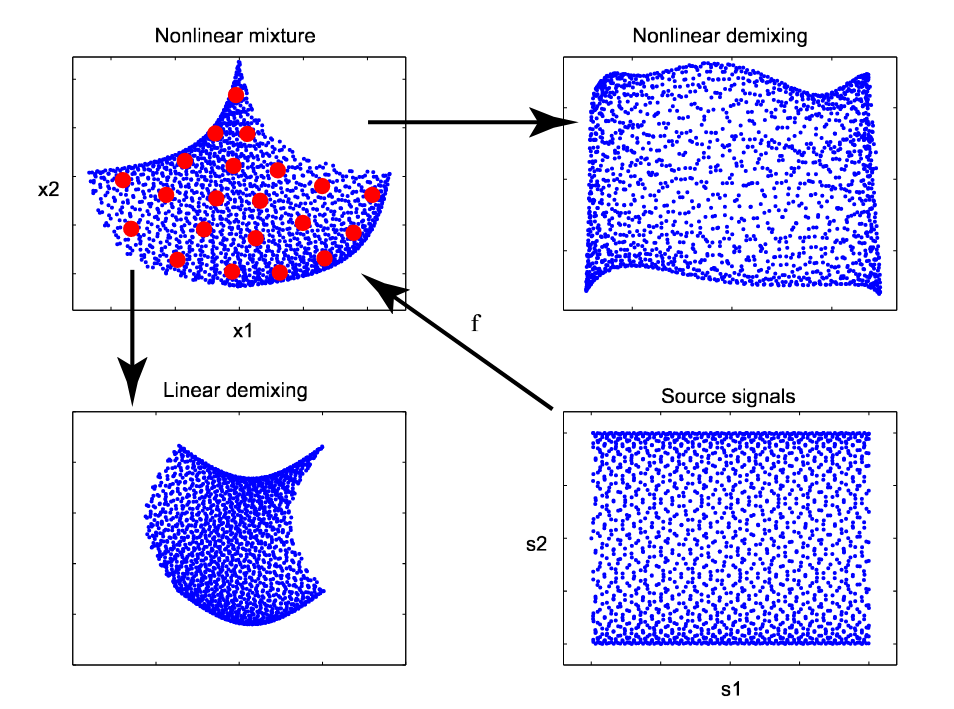
\includegraphics[scale=0.35]{Figures/Kernel.png}
	\caption{نتایج تجربی آزمایش تجربی الگوریتم 
		\lr{kTDSEP}
	}
	\label{kernel}
\end{figure}



\section{مدل‌های مشخص غیرخطی}
جداسازی کور منابع در مخلوط‌های غیرخطی برخی مخلوط‌های غیرخطی خاص تا کنون به خوبی مطالعه شده‌اند. در ادامه به صورت مختصر به بررسی این مدل‌ها می‌پردازیم.
\subsubsection{مدل‌های
	\lr{Post-Nonlinear}}
در این مدل‌ها، سیستم مخلوط‌کننده یک ماتریس است که در انتها هر درایه‌ی خروجی آن به صورت مولفه‌ به مولفه تحت یک تابع غیرخطی قرار گرفته است. این مدل در شکل 
\eqref{pnl}
دیده‌ می‌شود. 
\begin{figure}[h!]
	\centering
	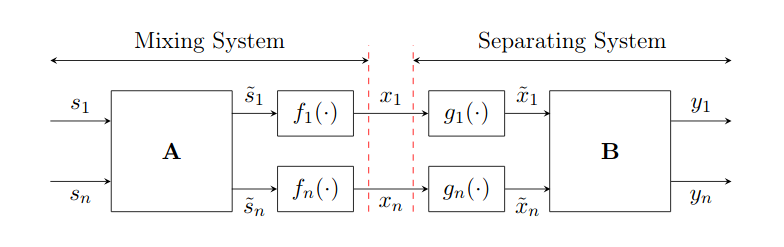
\includegraphics[scale=0.5]{Figures/pnl.png}
	\caption{مدل
		\lr{Post-Nonlinear}
	}
	\label{pnl}
\end{figure}

این مدل تاکنون به طور وسیع بررسی شده است و نشان جدایی‌پذیری آن اثبات شده است. الگوریتم‌های متعددی نیز تاکنون برای جداسازی این مخلوط‌ها ارائه گشته است. به عنوان نمونه می‌توانید مقاله‌ی 
\cite{pnl}
را ببینید. 

\subsubsection{مدل‌های خطی-مربعی}
سیستم مخلوط‌کننده در این مدل‌ها به فرم زیر در نظر گرفته می‌شود:
\begin{equation}
\forall 1\leq i\leq n \;\;\;\;
x_i = \sum_{j = 1}^{n} a_{ij}s_j + \sum_{j = 1}^{n}\sum_{k = j}^{n} b_{ijk} s_j s_k
\end{equation}
مشابه مدل‌های 
\lr{PNL}،
این مدل‌ها نیز به طور جدی مورد بررسی تئوری قرار گرفته‌اند و شرایط جدایی‌پذیری آن‌ها شناخته‌شده است
\cite{LQBSS}.

\chapter{تخمین مبتنی بر تفکیک نویز}
\label{chapter:NCE}
در این فصل به بررسی تخمین مبتنی بر تفکیک نویز\LTRfootnote{Noise Contrastive Estimation}
می‌پردازیم. این  روش، ایده‌ی برای تبدیل مسائل یادگیری نظارت‌نشده را به یادگیری نظارت‌شده در اختیار قرار می‌دهد. در فصل‌های آینده، از نتایج مطرح‌شده در این فصل برای مطالعه‌ی مخلوط‌های غیرخطی بهره می‌بریم. منبع اصلی در این فصل
\cite{NCE}
است.

\section{طرح مسئله}
فرض کنید
$\{P_{\boldsymbol{\theta}}: \boldsymbol{\theta} \in \boldsymbol{\Theta} \}$
 خانواده‌ای پارامتری از توزیع‌های احتمال بوده و 
 $\boldsymbol{\Theta}$
 مجموعه‌ی پارامتر‌های ممکن باشد. قصد داریم با مشاهده‌ی 
 نمونه‌های مستقل 
 $X_1, \dots, X_n \sim P_{\boldsymbol{\theta}^*}$،
 پارامتر 
 $\boldsymbol{\theta}^*$
 که از آن بی‌اطلاع هستیم را بیابیم. این مسئله، تخمین چگالی احتمال و یک مسئله‌ی یادگیری نظارت‌نشده است.

\section{تبدیل مسئله‌ به یک مسئله‌ی یادگیری نظارت‌شده}


برای حل مسئله‌ی بخش قبل، بدین شیوه عمل می‌کنیم: یک توزیع متفاوت و دلخواه مثل 
$P_n$
 در نظر گرفته و $n$ نمونه‌ی مستقل از آن تولید می‌کنیم. این نمونه‌ها را 
 $Y_1, \dots, Y_n$
 بنامید. حال، مجموعه‌ی 
 $$S = \{(X_1, 1), \dots, (X_n, 1),(Y_1, 0), \dots, (Y_n, 0)  \}$$
 را از داده‌های تولید شده و نمونه‌های توزیع ناشناخته، می‌سازیم. می‌خواهیم یک طبقه‌بند را به نحوی آموزش بدهیم که یک داده‌ از نمونه‌های 
 $X$
 یا 
 $Y$
 را گرفته و برچسب آن را در مجموعه‌ی $S$ به درسی تشخیص دهد. این روش، روش تخمین بر مبنای تفکیک نویز نام دارد.
 
 
   هر عضو مجموعه‌ی 
 $S$
 را با 
 $(U_t, C_t)$
 نشان می‌دهیم که 
 $t \in [2n]$.
توزیع داده‌های 
$X$
با فرض اینکه از یک توزیع با پارامتر
$\boldmath{\theta}$
 آمده‌اند، به صورت زیر مدل می‌شود:
 $$p(U_t = \u|C_t = 1; \boldsymbol{\theta}) = p_{\boldsymbol\theta} (\u)،$$
 همچنین
 $$p(U_t = \u|C_t = 0) = p_n (\u).$$
 
 توزیع پیشین $C$ نیز برابر 
 $P(C_t = 1) = 1 - P(C_t = 0) = \frac{1}{2}$
 است. با توجه به این توزیع‌ها و با قانون بیز، در‌می‌یابیم که
 
\begin{equation}
P(C_t = 1 | U_t = \u; \boldsymbol{\theta}) = \frac{p_{\boldsymbol{\theta}}(\u)}{p_{\boldsymbol{\theta}(\u)} + p_n(\u)}
\end{equation}
و 
\begin{equation}
P(C_t = 0 | U_t = \u; \boldsymbol{\theta}) = \frac{p_{n}(\u)}{p_{\boldsymbol{\theta}(\u)} + p_n(\u)}.
\end{equation}


تابع $G$ را به عنوان اخختلاف لگاریتم دو چگالی احتمال تعریف می‌کنیم:
 \begin{equation}
G(\u, \boldsymbol{\theta}) \triangleq \ln p_{\boldsymbol{\theta}}(\u) - \ln p_n (\u).
 \end{equation}
 
 با این تعریف،  داریم
 \begin{equation}
h(\u; \boldsymbol{\theta}) \triangleq P(C_t = 1 | U_t = \u; \boldsymbol{\theta})= r\big(G(\u, \boldsymbol{\theta})\big)
 \end{equation}
 که در آن $r$ تابع لاجستیک، یعنی 
$
r(s) = \frac{1}{1 + \exp(-s)}
$
است. با توجه به این تعارف، می‌توان اگاریتم تابع لایکلیهود شرطی را به فرم زیر نوشت
\begin{align*}
l_n(\boldsymbol\theta) &= \sum_{t = 1}^{2n} C_t \ln P(C_t = 1 | \u_t, \boldsymbol\theta) + (1- C_t)\ln P(C_t = 0 | \u_t, \boldsymbol\theta)\\
&=\sum_{t= 1}^{n}\ln[h(\x_t; \boldsymbol\theta)] + \sum_{t = 1}^{n} \ln[1 - h(\y_t; \boldsymbol{\theta})].
\end{align*}

تعریف می‌کنیم 
$J_n(\boldsymbol{\theta}) \triangleq \frac{l(\boldsymbol{\theta})}{n} $.
یک الگوریتم طبیعی برای به دست آوردن 
$\boldsymbol{\theta}$،
استفاده از الگوریتم بیشینه‌کردن تابع لایکلیهود است، یعنی
\begin{equation}
\hat{\boldsymbol{\theta}}_n = \arg\max_{\boldsymbol{\theta} \in \boldsymbol{\Theta}} l_n(\boldsymbol{\theta}) = \arg\max_{\boldsymbol{\theta} \in \boldsymbol{\Theta}} J_n(\boldsymbol{\theta}).
\end{equation}

در ادامه نشان خواهیم داد که این تخمین‌گر، تخمین‌گر مناسبی است.

\begin{theorem}
	با افزایش $n$، داریم
\begin{equation}
J_n(\boldsymbol{\theta}) \rightarrow J(\boldsymbol\theta)
\hspace{1cm}
\text{در احتمال}
\end{equation}
که در آن
$$
J(\boldsymbol\theta) = \E_\x\Big[\ln[h(\x, \boldsymbol\theta)]\Big] + \E_\y\Big[\ln[1 - h(\y, \boldsymbol\theta)]\Big].
$$
\end{theorem}
\begin{proof}
نتیجه‌ی مستقیم قانون ضعیف اعداد بزرگ.
\end{proof}


یک راه مناسب بررسی عملکرد الگوریتم مطرح‌شده، آن است که چشم‌انداز بهینه‌سازی \LTRfootnote{Optimization Landscape}
را بر حسب تابع
$f(.) = \ln p_{\boldsymbol{\theta}}(.)$
مطالعه کنیم. یعنی ببینیم که با تغییرات در تابع 
$f$،
تابع هزینه‌ در الگوریتم (لایکلیهود شرطی)، چگونه تغییر می‌کند. تابع $\tilde{J}(f)$ را به عنوان تابع $J$ بر حسب $f$ تعریف می‌کنیم:
\begin{equation}
\tilde{J}(f) = \E_\x\Big[\ln\big(r(f(\x) - \ln p_n(\x)\big)\Big] + \E_\y\Big[\ln\big(1 - r(f(\y) - \ln p_n(\y)\big)\Big].
\end{equation}

\begin{theorem}
	\label{fth}
	اگر تابع چگالی احتمال
	$p_n$
	به نحوی باشند که در هر جا که 
	$p_{\boldsymbol{\theta}^*}$
	صفر نیست، صفر نباشد، آن‌گاه تابع 
	$\tilde{J}$
	مقدار بیشینه‌ی خود را در 
	$f = \ln p_{\boldsymbol{\theta}^*}$
	اخذ می‌کند.
	
\end{theorem}

\begin{proof}
اثبات ساده است و در  
\lr{Appendix A}
مقاله‌ی
\cite{NCE}
موجود است.
\end{proof}

\begin{theorem}
	 اگر شروط (۱) تا (۳) برقرار باشند، با افزایش 
$n$
تخمین‌گر
$\hat{\boldsymbol\theta}_n$
در احتمال به 
$\boldsymbol{\theta}^*$
میل می‌کند.

\begin{itemize}
\item 
$p_n$
در هر جا 
$p_{\boldsymbol{\theta}^*}$
ناصفر است، صفر نیست.

\item 
$\sup_{\boldsymbol{\boldsymbol\theta}} |J_n(\boldsymbol\theta) - J(\boldsymbol{\theta})|$
در احتمال به صفر میل کند.

\item 
ماتریس
$\mathcal{I} = \int g(\u) g(\u)^T P(\u) p_{\boldsymbol{\theta}^*}(\u) d\u$
دارای رتبه‌ی کامل است. که در این ماتریس
\begin{equation}
g(\u) \triangleq \nabla_\theta p_{\boldsymbol{\theta}^*}(\u)
\end{equation}
و
\begin{equation}
P(\u) \triangleq \frac{p_n(\u)}{p_{\boldsymbol{\theta}}^*(\u) + p_n(\u)}.
\end{equation}

\end{itemize}
\end{theorem}

\begin{proof}
صورت و اثبات این قضیه، کاملاً مشابه اثبات قضیه‌ی معروف همگرایی تخمین ماکزیمم لایکلیهود در حالت کلی است. آن اثبات، در مقالات و کتب آمار کلاسیک یافت می‌شود. به عنوان مثال 
\cite{wasserman}
را ببینید.  آن قضیه در فصل ۹، قضیه‌ی ۱۳ آورده شده است.

 شرط اول  از قضیه‌ی
\eqref{fth}
به ارث می‌رسد. شرط دوم، معادل شرط همگرایی یکنواخت\LTRfootnote{Uniform Convergance}
تابع لاگ لایکلیهود به دیورژانس کوبلک-لایبلر در قضیه‌ی اصلی همگرایی تخمین ماکزیمم لایکلیهود است و شرط سوم هم معادل شرط (۹.۸) کتاب 
\cite{wasserman}
است.
\end{proof}

\chapter{جدایی‌پذیری مخلوط‌های غیرخطی}
\label{seprability}
در این بخش به بررسی قضایای مربوط به جدایی پذیری مخلوط‌های غیرخطی می‌پردازیم. در ابتدا با یک مثال نشان می‌دهیم که همه‌ی مخلوط‌های غیرخطی فرآیند‌های تصادفی مستقل، جدایی‌پذیر نیستند.

\begin{example}
	
	
	فرآیند‌های تصادفی ورودی
$
\begin{cases}
s_1[i] = s_1[i-1] + \mathcal{N}(0,1)\\
s_2[i] = s_2[i-1] + \mathcal{N}(0,1)
\end{cases}
$
	و تابع مخلوط‌کننده‌ی  وارون‌پذیر
$ f\big([s_1, s_2]^\top\big)= 
\begin{bmatrix}
s_1\\
\mathrm{sign}(s_1s_2)
\end{bmatrix}
$
را در نظر بگیرید. به سادگی می‌توان دید که فرآیند‌های تصادفی حاصل از اعمال تابع مخلوط‌کننده بر فرآیندهای تصادفی فوق، از یکدیگر مستقل هستند.
\end{example}

\section{
	روش تمایز بین زمان‌ها
	\lr{(TCL)}
}
روش تمایز بین زمان‌ها یا 
\lr{Time-Contrastive Learning (TCL)} 
روشی است برمبنای آموزش یک استخراج‌گر ویژگی\LTRfootnote{Feature Extractor} با استفاده از یک طبقه‌بند\LTRfootnote{Classifier}
\lr{Multinomial Logistic Regression}
که می‌خواهد بین قطعه‌های زمانی سیگنال زمانی، تفکیک قائل‌شود. این روش در 
\cite{TCL}
معرفی شده‌است. در این بخش، در ابتدا به معرفی 
\lr{TCL}
پرداخته و سپس نشان می‌دهیم این روش می‌تواند دسته‌ای از مسائل جداسازی کور مخلوط‌های غیرخطی را حل نماید.

\subsection{الگوریتم 
	TCL
}

الگوریتم زیر را در نظر بگیرید:

\begin{enumerate}%\def\labelenumi{A\theenumi)}
	\setlength{\itemsep}{-0.5mm}%\setlength{\paraindent}{0mm}
	\item 
	سیگنال‌های زمانی 
	$\x(t)$
	را به تعدادی سگمنت‌ زمانی تقسیم کنید. (پنجره‌های زمانی که اندیس آن‌ها $\tau=1,\ldots,T$) است. طول این پنجره‌ها را برابر در نظر بگیرید. فرض کنید در هر پنجره‌ی زمانی، $L$ استپ زمانی داریم.
	\item 
	مقادیری از سیگنال 
	$\x(t)$
	که در بازه‌ی زمانی 
	$\tau$
	قرار دارد، برچسب 
	$\tau$
	بدهید. اگر در هر سگمنت $L$ استپ زمانی داشته باشیم، برای هر برچسب در دیتاست تولید شده، $L$ نمونه داریم. هر یک از این نمونه‌ها یک بردار $n$ بعدی است ($\x(i)$).
	
	\item
	یک استخراج‌گر ویژگی 
	$\mathbf{h}(\x_t;\thetab)$ 
	و یک 
	\lr{MLR}
	را برای طبقه‌بندی دیتاستی که در مرحله‌ی تولید کرده‌اید آموزش دهید. برای 
	\lr{MLR}
	از تابع رگرسیون 
	$ w_\tau^T \h(\x_t; \thetab)+b_\tau$
	استفاده نمایید.
	
\end{enumerate}

در این جا هدف استخراج‌گر ویژگی آن است که ویژگی‌هایی از داده بیابید که به 
\lr{MLR}
کمک کند طبقه‌بندی بهتری انجام دهد.  شهوداً می توان انتظار داشت که این استخراج‌گر باید نمایش مناسبی از سیگنال و رابط زمانی موجود در آن ر ا یاد بگیرد. در عمل، از آن‌جا که انتظار داریم تابع 
$\h$
توانایی تقریب هر تابع غیرخطی را داشته باشد، از یک 
\lr{MLP}
با حذف لایه‌ی آخر آن، به عنوان $\h$ استفاده می‌کنیم. در بخش بعد اثبات می‌‌کنیم که این استخراج‌گر ویژگی، در عمل، جداسازی کور منابع را انجام داده است. شکل 
\eqref{TCL}،
روند کلی این روش را نمایش می‌دهد.
\begin{figure}
	\centering
	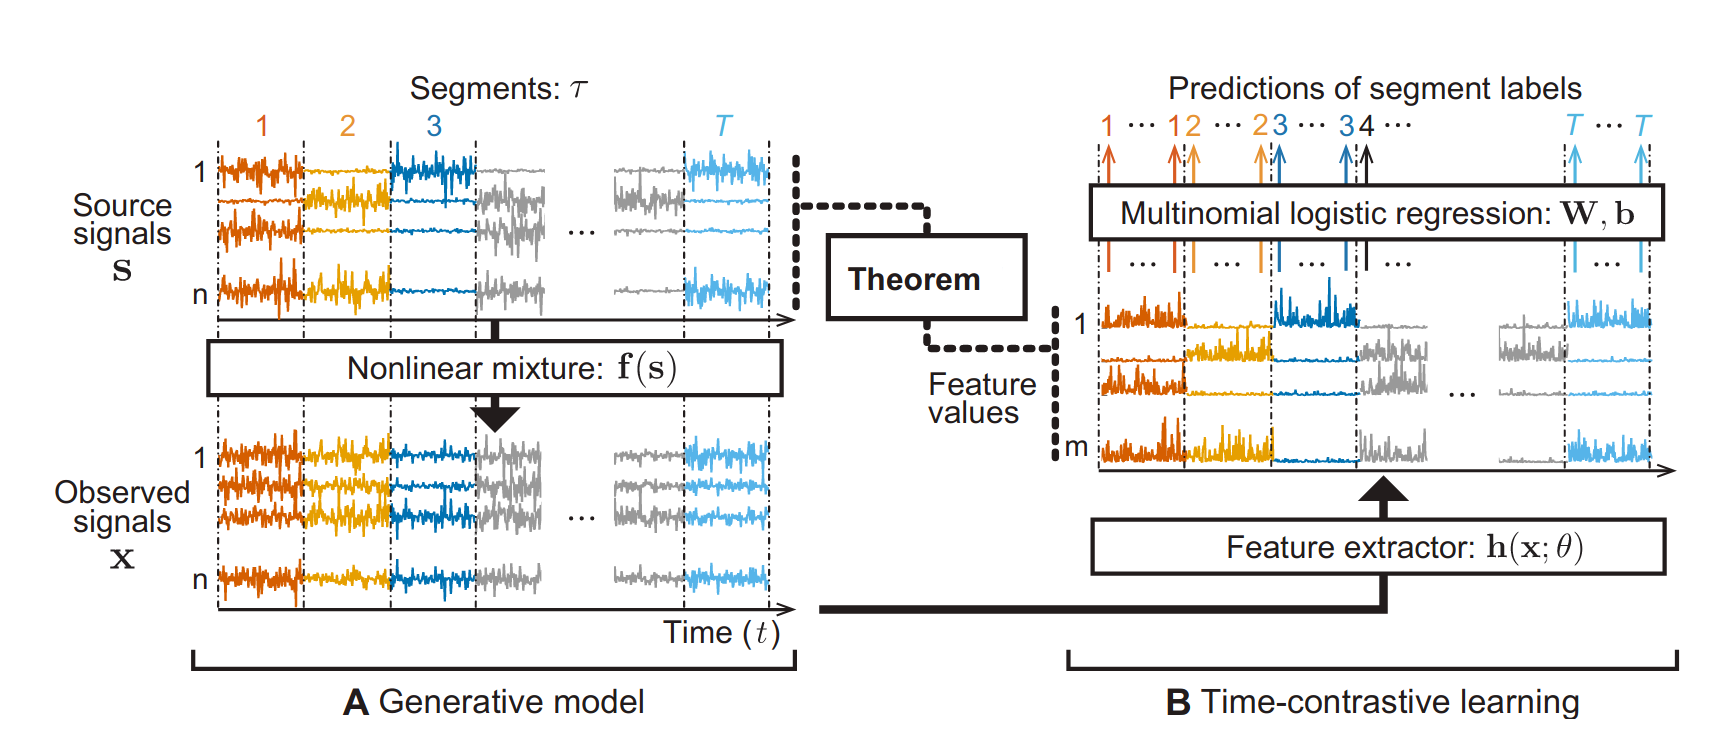
\includegraphics[scale=1.1]{Figures/TCL.png}
	\caption{شمای کلی روش تمایز بین زمان‌ها
		(TCL)
	}
	\label{TCL}
\end{figure}

\subsection{
	\lr{TCL}
	به عنوان تقریبی از نسبت
	\lr{log-pdf}
	ها
}

در یک 
\lr{MLR}،
احتمال
\lr{posterior}
برای اینکه دیتای 
$\x_t$
عضو دسته‌ی 
$\tau$
باشد، برابر است با:
\begin{align}
%    \ell(\thetab, \m W, \ve b) = 
p(C_t=\tau | \x_t; \thetab,  \mathbf {W},  \mathbf {b})= 
%\nonumber \\
\frac{\exp( w_\tau^T \h(\x_t; \thetab)+b_\tau)}
{1+\sum_{j=2}^{T} \exp( w_j^T \h(\x_t; \thetab)+b_j)}  \label{eq:ell2}
\end{align}
که در آن 
$C_t$
برچسب دیتا در زمان 
$t$،
$\x_t \in \R^n$
بردار دیتا در زمان $t$،
$\theta$
پارامتر‌های استراج‌گر ویژگی،
$\mathbf{W} = [\mathbf{w}_1, \mathbf{w}_2, \dots, \mathbf{w}_T] \in 
\R^{m \times T}$
وزن‌ها 
و 
$\mathbf{b} = [b_1, \dots b_T]^\top$
بایاس‌های 
\lr{MLR}
هستند. از طرف دیگر، با قانون بیز، می‌توان نوشت:
\begin{equation}
p(C_t=\tau | \x_t) = \frac{p_\tau(\x_t)p(C_t = \tau)}
{\sum_{j=1}^{T} p_j(\x_t)p(C_t = j)},
\label{eq:pc_i}
\end{equation}
که در آن 
$p(C_t = \tau)$
توزیع پیشین برچسب یک سگمنت است و 
$p_\tau(\x_t) = p(\x_t| C_t = \tau)$
است. اگر استخراج‌گر ویژگی، ویژگی
\lr{Universal Approximation Capacity}
را داشته و بیشمار داده در اختیار باشد، 
\eqref{eq:ell2}
به 
\eqref{eq:pc_i}
همگرا می‌شود. با مساوی قرار دادن این دو عبارت، داریم:
\begin{equation} 
w_\tau^T \h(\x_t; \thetab) + b_\tau 
= \log p_\tau(\x_t) - \log p_1(\x_t) + \log \frac{p(C_t = \tau)}{p(C_t = 1)} ,
\label{eq:relation}
\end{equation}

اگر طول سگمنت‌ها برابر باشد، عبارت سومین جمله‌ی سمت راست تساوی نیز برابر با صفر می‌شود، در نتیجه:
\begin{equation} 
w_\tau^T \h(\x_t; \thetab) + b_\tau 
= \log p_\tau(\x_t) - \log p_1(\x_t)
\label{eq:relation2}
\end{equation}

\subsection{	استفاده از
	\lr{TCL}
	در جداسازی کور منابع}
مجدداً مدل مطرح شده در فصل
\eqref{probdef}
را در نظر بگیرید:
\begin{equation}
\s_t = \big(s_1(t), s_2(t), \dots, s_n(t)\big);\;\;\;\;
\x_t = \mathbf{f}(\s_t)
\end{equation}
فرض‌کنید سیگنال‌های 
$s_i(t)$
غیر ایستان باشند.  همچنین 
$s_i(t)$
ها را فرآیندهایی مشترکاً مستقل در نظر بگیرید. فرض کنید، غیر ایستان بودن فرآیند‌ها آنقدر کند است که می‌توانیم توزیع را در هر سگمنت از دیتا ثابت بگیریم. 
\lr{log-pdf}
منبع با اندیس 
$i$
در سگمنت
$\tau$
را به صورت زیر تعریف می کنیم:
\begin{equation} 
\log p_\tau(s_i)=  q_{i,0}(s_i) + \sum_{v=1}^V \lambda_{i,v}(\tau) q_{i,v}(s_i) - \log Z( \lambda_{i,1}(\tau),\ldots,\lambda_{i,v}(\tau))
\label{eq:p_tau}
\end{equation}
اندیس $t$ برای سادگی حذف شده‌است.
در این عبارت،
$q_{i, 0}$
یک
\lr{stationary baseline}
برای توزیع منابع است. توابع 
$q_{i, v}$
به ازای 
$ v\geq 1$
توابع غیرخطی اسکالری هستند که تابع 
$\tau$
بوده و مدل‌کننده‌ی غیر ایستان بودن منبع هستند.
$Z$
نقش نرمالایز کننده‌ی توزیع احتمال را بر عهده دارد که در تمامی اثبات‌ها حذف می‌شود و بی‌اثر است.

\begin{example}
	برای مثال، فرض کنید 
	$q_{i, 0} = 0$
	است و $V$ را برابر یک در نظر بگیرید. تابع
	$q_{i, 1} (s_i) = -\frac{s_i^2}{2}$
	مدل کننده‌ی یک منبع گوسی است که واریانس آن در حال تغییر است. اگر 
	$q_{i, 1} (s_i) = -|s_i|$
	در نظر می‌گرفتیم، منبع یک منبع لاپلاسی می‌شد.
\end{example}

حال می‌خواهیم به بررسی روش استفاده از 
\lr{TCL}
برای حل جداسازی کور بپردازیم.

\begin{theorem}
	در مدل 
	\eqref{eq:p_tau}
	فرض کنید 
	$V = 1$
	است،
	$q_{i, 0} = 0$
	و
	$q \triangleq q_{i, 1}$،
	یعنی منابع به صورت زیر تولید شده‌اند:
	\begin{equation}
	\log p_\tau(s_i)=    \lambda_{i,1}(\tau) q(s_i) - \log Z( \lambda_{i,1}(\tau))
	\label{eq:p_tau_simple}
	\end{equation}
	\begin{itemize}
		\item
		فرض کنید 
		\lr{TCL}
		را بر  روی دیتای تولیدشده از مدل فوق اعمال کنیم و در آن، بُعد استخراج‌گر ویژگی، 
		$\h$
		را برابر تعداد منابع (که برای تعداد سری‌های زمانی مشاهده‌شده است) در نظر بگیریم. 
		\item
		فرض کنید ماتریس 
		$\mathbf{L}$
		با المان‌های 
		$$[\mathbf{L}]_{\tau, i} = 
		\lambda_{i, 1}(\tau) - \lambda_{i, 1}(1) \
		\;\;\;\;
		\tau = 1, \dots, T, \;\;
		i = 1, \dots, n
		$$
		داری رتبه‌ی ستونی کامل باشد\footnote{
			توجه کنید که از آن‌جایی که ماتریس 
			$\mathbf{L}$
			یک ماتریس بلند است و حتی با فرض مذکور، سگمنت‌های زمانی زیادی می‌توانند توزیع یکسانی داشته باشند.}.
	\end{itemize}
	در این حالت، در حدی که بیشمار نمونه‌ی زمانی از فرآیند های تصادفی در اختیار داشته داریم، ماتریس 
	$\mathbf{A} \in \R^{n\times n}$
	و
	$\mathbf{d} \in \R^n$
	وجود دارند که:
	\begin{equation}
	q(\s_t) = \mathbf{Ah}(\x_t, \theta) + \mathbf{d}
	\end{equation}
\end{theorem}

\begin{note}
	شهود کامل بودن رتبه‌ی ماتریس 
	$\mathbf{L}$
	این است که واریانس منابع، مستقل از یکدیگر در حال تغییر هستند.
\end{note}
\begin{proof}
	در ابتدا، توزیع احتمال 
	$\x_t$
	را بر حسب توزیع احتمال
	$\s_t$
	به دست می‌آوریم:
	\begin{equation}
	\log p_\tau(\x) = \sum_{i=1}^n \lambda_{\tau,i}q(g_i(\x)) 
	+ \log | \det  \mathbf{J} \mathbf{g} (\x) | - \log Z(\lambda_\tau),
	\label{eq:p_x}
	\end{equation}
	در این عبارت، برای سادگی از اندیس 
	$t$ 
	برای
	$\x$
	چشم پوشی کرده‌ایم. همچنین
	\begin{equation}
	\mathbf{g}(\x) = \big(g_1(\x), g_2(\x), \dots, g_n(\x)\big)^\top
	\end{equation}
	تابع وارون مخلوط‌کننده‌ی
	$\mathbf{f}$
	است (یعنی بنا بر تعریف
	$s_i = g_i(\x)$).
	ماتریس 
	$\mathbf{Jg}$
	نیز ژاکوبین تبدیل 
	$\mathbf{g}$
	است. با استفاده از 
	\eqref{eq:relation}
	می‌توان نوشت:
	\begin{equation} 
	\log p_\tau(\x)= \sum_{i=1}^n w_{\tau,i} h_i(\x) + b_\tau + \log p_1(\x) - c_\tau,
	\label{eq:optlrpdfbias}
	\end{equation}
	در این معادله، 
	$w_{\tau, i}$
	و
	$h_i{\x}$،
	المان‌های 
	$i$ام
	بردار‌های 
	$\mathbf{w}_\tau$
	و
	$\mathbf{h}(\x)$
	هستند. در این عبارت، پارامتر‌های
	$\theta$
	در 
	$\mathbf{h}$
	را برای سادگی حذف کرده‌ایم. 
	$c_\tau$
	نیز عبارت آخر در سمت راست
	\eqref{eq:relation}
	است. با قرار دادن 
	$\tau = 1$
	در 
	\eqref{eq:p_x}
	داریم:
	\begin{equation}
	\log p_1(\x)= \sum_{i=1}^n \lambda_{1,i} q(g_i(\x)) + \log |\det \mathbf{ J g}(\x)| - \log Z(\lambda_1).
	\label{eq:p1_x}
	\end{equation} 
	با جای‌گذاری این عبارت در 
	\eqref{eq:optlrpdfbias}
	داریم:
	\begin{align} \label{eq:optlrpdf2}
	\log p_\tau(\x) = \sum_{i=1}^n \left[w_{\tau,i} h_i(\x) + \lambda_{1,i} q(g_i(\x)) \right] \\
	+ \log |\det\mathbf{ J g}(\x)| - \log Z(\lambda_1)  + b_\tau - c_\tau.
	\end{align}
	
	با مساوی قرار دادن 
	\eqref{eq:optlrpdf2}
	و
	\eqref{eq:p_x}
	به ازای هر 
	$\tau$
	داریم:
	\begin{equation}
	\sum_{i=1}^n \tilde{\lambda}_{\tau,i} q(g_i(\x)) 
	= \sum_{i=1}^n w_{\tau,i} h_i(\x) + \beta_\tau,
	\label{eq:maineq}
	\end{equation}
	در این معادله داریم
	$\tilde{\lambda}_{\tau,i}= \lambda_{\tau,i}- \lambda_{1,i}$ 
	و
	$\beta_\tau= \log Z(\lambda_\tau)-\log Z(\lambda_1)+b_\tau-c_\tau$.
	با نوشتن این معادله‌ها برای 
	$\tau$
	های مختلف  به فرم ماتریس داریم:
	\begin{equation}
	\mathbf{ L} q(\s) %\begin{pmatrix} q(s_1)\\ q(s_2)\\ \vdots\\ q(s_n) \end{pmatrix} 
	= \mathbf{W} \h(\x) + \mathbf{\beta}
	\end{equation}
	در این معادله،
	$\mathbf{ L}$
	همان ماتریس صورت قضیه است،
	$\mathbf{ W}$
	فرم ماتریسی
	$w_{\tau, i}$
	و
	$\mathbf{\beta}$
	بردار 
	$\beta_\tau$
	هاست.
	
	با توجه به این‌که ماتریس
	$\mathbf{ L}$
	دارای رتبه‌ی ستونی کامل است، برای شبه-وارون آن داریم
	$\mathbf{L}^+\mathbf{L} = \mathbf{I}$. 
	با ضرب شبه-وارون در عبارت آخر به 
	\begin{equation}
	q(\s)
	%\begin{pmatrix} q(s_1)\\ q(s_2)\\ \vdots\\ q(s_n) \end{pmatrix} 
	= [\mathbf{L}^+  \mathbf{W}] \h(\x) + \mathbf{L}^+ \beta.
	\end{equation}
	می‌رسیم. که معادل گزاره‌ی صورت سوال است که در آن 
	$\mathbf{A} = \mathbf{L}^+  \mathbf{W}$
	یک ماتریس وارون‌پذیر است. اگر رتبه‌ی این ماتریس کامل نبود، توابع 
	$q(s_i)$
	وابسته‌ی خطی می‌بودند، که غیرممکن است زیرا تابع متغیر‌های 
	$s_i$
	هستند.
\end{proof}

\begin{corollary}
	فرض‌ کنید
	$\lambda_{i, 1}$
	ها به صورت تصادفی تولید شده‌باشند. جدا کردن منابع 
	$s_i$
	می‌تواند با اعمال 
	\lr{TCL}
	و سپس اعمال یک الگوریتم خطی جداسازی کور بر روی خروجی‌های استخراج‌گر ویژگی
	$\mathbf{h}$
	ا نجام بگیرد، زیر $q$ یک کران بالا دارد (به خاطر انتگرال‌پذیر بودن) و در نتیجه 
	$q(s_i)$
	غیر گوسی است.
	\label{corr}
\end{corollary}

\begin{note}
	در حالت کلی، تابع $q$ وارون‌پذیر نیست و از نتیجه‌ی
	\eqref{corr}
	نمی‌توان برای جداسازی 
	$s_i$
	ها استفاده کرد.
\end{note}
\begin{corollary}
	فرض کنید 
	$q(s)$
	تابعی اکیداً یکنوا از 
	$|s|$
	باشد. در این صورت،  $s_i$ ها «قابل بازسازی» هستند.
\end{corollary}
\begin{proof}
	برای انتگرال‌پذیر بودن
	$p_\tau(s)$،
	باید در حد
	$|s| \to \infty$،
	تابع
	$q(s) \to -\infty$
	برود.  در ضمن،
	$q(s)$
	باید یک ماکزیمم محدود داشته باشد. بدون کم شدن از کلیت مسئله، این ماکزیمم را برابر صفر در نظر بگیرید. برای یک $i$ مشخص، منیفلد
	$q(g_i(\x)) = 0$
	را در نظر بگیرید. این منیفلد، فضای 
	$\x$
	را به یک بخش با 
	$\tilde{s_i} = q(s_i)$
	و یک بخش با 
	$\tilde{s_i} = -q(s_i)$
	تقسیم می‌کند. با این 
	$\tilde{s_i}$،
	ما منابع را در حد یک تابع یکنوا بازسازی کرده‌ایم:
	$\tilde{s_i} = c \;\mathrm{sign}(s_i)q(s_i)$
	که در آن 
	$c \in \{-1, +1\}$.
\end{proof}

\section{استفاده از متغیر‌های کمکی}

ایده‌ی اصلی این روش‌ها این است که اگر 
$n$
منبع وجود داشته باشند، $m$ متغیر 
$\u$
را به نحوی انتخاب می‌کنند که توابع 
$q_i$
وجود داشته باشند به نحوی که:
\begin{equation}
\log p(\s|\ub) = \sum_{i = 1}^{n} q_i(s_i, \ub)
\label{genprior}
\end{equation}
این ایده‌ می‌تواند تعمیم ایده‌ی 
\lr{(TCL)}
در نظر گرفته شود که در آن از شماره‌ی سگمنت به عنوان متعیر 
$\ub$
استفاده می‌شد. ایده‌ این است که مجدداً یک دیتاست بسازیم:
\begin{align}
\xaug=(\x,\uu)  \  \text{ vs. } \
\xaug^*=(\x,\uu^*) \label{xtildestar}
\end{align}
در این‌جا 
$\uu^*$
هم‌توزیع با 
$\uu$
است، اما از 
$\x$
مستقل است. در عمل 
$\uu^*$
را با جایگشت دادن نمونه‌های 
$\uu$
می‌سازیم. یک
\lr{Logistic Regression}
را با تابع رگرسیون
\begin{equation} \label{reggen}
r(\x,\uu)= \sum_{i=1}^n \psi_i(h_i(\x),\uu)
\end{equation}
یاد می‌گیریم که به ما احتمال این‌که یک بردار 
$\x$
و 
$\uu$
داده‌شده  در کلاس اول یا کلاس دوم باشند را می‌دهد. احتمال این که در کلاس اول باشد، برابر است با
$1/(1+\exp(-r(\x,\uu))$.
فرض می‌کنیم که 
$h_i$
ها و 
$\psi_i$
ها ویژگی
\lr{Universal Approximation Capacity}
را داشته باشند. در ادامه به بیان دقیق قضیه‌ی جدایی‌پذیری  می‌پردازیم:

\begin{theorem}
	فرض کنید:
	\begin{enumerate}
		\item 
		فرض کنید داده از مدل غیرخطی
		$\x = \f(\s)$
		تولید می‌شود و رابطه‌ی 
		\eqref{genprior}
		برقرار است.
		\item
		به ازای هر 
		$\uu$
		توابع 
		$q_i$
		به عنوان تابعی از 
		$s_i$
		به اندازه‌ی کافی هموار هستند.
		\item
		برای هر بردار 
		$\y \in \R^n$،
		تعداد 
		$2n+1$
		مقدار برای 
		$\uu$
		وجود دارد که با 
		$\uu_i$
		نمایش داده‌شده اند. این بردار‌ها به گونه‌ای هستند که
		$2n$
		بردار
		\begin{multline}
		\left(\w(\y,\uu_1)-\w(\y,\uu_0)),(\w(\y,\uu_2)-\w(\y,\uu_0)),\right. \\ \left. ...,(\w(\y,\uu_{\ncond})-\w(\y,\uu_0)\right)
		\end{multline}
		که عضو
		$\R^{2n}$
		هستند و در آن‌ها 
		\begin{multline} \label{wdef}
		\w(\y,\uu)=\left(\frac{\partial q_1(y_1,\uu)}{ \partial y_1},\ldots,\frac{\partial q_n(y_n,\uu)}{ \partial y_n},  \right. \\ \frac{\partial^2 q_1(y_1,\uu)}{ \partial y_1^2},   \left. \ldots,\frac{\partial^2 q_n(y_n,\uu)}{ \partial y_n^2}\right)
		\end{multline}
		است، مستقل خطی باشند.
		\item 
		یک رگرسون لاجیستیک
		با  
		\lr{Universal Approximation Capacity}
		را آموزش می‌دهیم تا بین 
		$\xaug$
		و
		$\xaug^*$
		تمایز قائل شود.
		\item
		فرض می‌کنیم توابع 
		$
		r(\x,\uu)= \sum_{i=1}^n \psi_i(h_i(\x),\uu)
		$
		هموار و وارون‌پذیر بوده و وارون آن‌ها نیز هموار باشد.
	\end{enumerate}
	در این صورت، در حدی که بیشمار داده در اختیار داریم، 
	$h_i(\x)$
	برابر منابع مستقل با حداکثر اعمال یک تابع  وارون‌پذیر هستند.
	\label{newthm}
\end{theorem}
\begin{proof}
	در این‌جا، از آوردن اثبات این قضیه چشم‌پوشی کرده‌ایم. اثبات این قضیه در بخش اول فصل
	\lr{Supplementary Material}
	مقاله‌ی 
	\cite{newHyva}
	آمده است.
\end{proof}

\begin{definition}
	متغیر تصادفی 
	$s_i$
	به شرط 
	$\uu$
	دارای توزیع نمایی شرطی از مرتبه‌ی 
	$k$
	است، اگر 
	\lr{pdf}
	آن به ازای هر 
	$\uu$
	قابل نوشتن به فرم زیر باشد:
	\begin{equation} \label{expdef}
	p(s_i|\uu)=\frac{Q_i(s_i)}{Z_i(\uu)}\exp[\sum_{j=1}^k \suffstat_{ij}(s_i)\lambda_{ij}(\uu)]
	\end{equation}
	در این معادله،
	$Q_i$،
	$\lambda_{ij}$،
	$\tilde{q}_{ij}$
	و 
	$Z_i$
	توابعی اسکالر هستند.
\end{definition}
\begin{example}
	در هر زمان داده‌شده، مقدار یک فرآیند تصادفی گوسی با 
	$\uu$
	ای برابر گذشته‌ی این فرآیند در این زمان، یک متغیر تصادفی نمایی شرطی با پارامتر 
	$k = 1$
	است.
\end{example}

\begin{theorem}
	اگر منابع
	$s_i$
	به شرط 
	$\uu$
	دارای توزیع شرطی نمایی با مرتبه‌ی 
	$k$
	باشند. در صورتی که  $k=1$ باشد، شرط سوم قضیه‌ی 
	\eqref{newthm}
	نمی‌تواند برقرار باشد.
\end{theorem}
\begin{proof}
	اثبات این قضیه در بخش دوم فصل
	\lr{Supplementary Material}
	مقاله‌ی 
	\cite{newHyva}
	آمده است.
\end{proof}
\begin{note}
	قضیه‌ی فوق، مشابه جدایی‌ناپذیر بودن متغیر‌های تصادفی گوسی در حالت خطی است.
	
	\section{استفاده از مشتق منابع}
	فرض کنید منابع 
	$\s$
	به صورت غیر خطی با یکدیگر مخلوط‌ شده باشند:
	\begin{equation}
	\x(t) = \f(\s(t))
	\end{equation}
	در این حالت، با وجود غیرخطی بودن تابع 
	$\f$،
	مشتق منابع در هر لحظه‌ به صورت خطی با یکدیگر مخلوط شده‌اند و مشتق سیگنال‌های 
	$\x$
	را تولید می‌کنند:
	\begin{equation}
	\frac{dx_i}{dt} = \sum_{j = 1}^{n} \frac{\partial f_i}{\partial s_j} \frac{ds_j}{dt}
	\implies
	\nabla\x = \mathbf{J}_{\f; t}(\s)\nabla\s
	\end{equation}
	که در آن، ماتریس 
	$ \mathbf{J}_{\f; t}$
	برابر ژاکوبین تبدیل 
	$\f$
	در نقطه‌ی 
	$\s(t)$
	است. 
	\begin{figure}[h!]
		\centering
		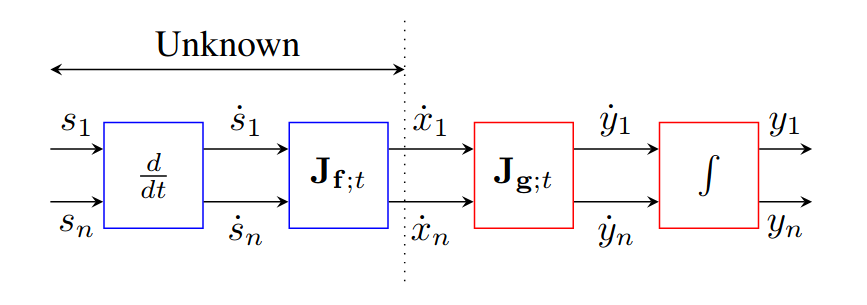
\includegraphics[scale=0.4]{Figures/ehsan.png}
		\caption{بهره‌بردن از مشتق برای جداسازی مخلوط‌های غیرخطی}
		\label{ehsan}
	\end{figure}
	
	این ایده برای اولین بار در مقاله‌ی 
	\cite{ehsandoust}
	مطرح شده است. ممکن است به نظر برسد که بر مبنای این ایده‌، و با توجه به قضیه‌ی جدایی‌پذیری مخلوط‌های خطی، به سادگی می‌توان قضیه‌ای برای جدایی‌پذیری مخلوط‌های غیرخطی مطرح کرد، اما این‌گونه نیست زیرا در این‌جا، ماتریس
	$ \mathbf{J}_{\f; t}$
	تابعی از زمان است و ثابت نیست. با این وجود، می‌توان بر مبنای این ایده و با فرض اینکه تغییرات ماتریس ژاکوبین در زمان بسیار کند است، الگوریتمی وفقی برای جداسازی کور مخلوط غیرخطی ارائه داد که تغییرات کند ماتریس ژاکوبین را دنبال کند. این روند در 
	\cite{ehsandoust}
	پی گرفته شده و الگوریتمی برای جداسازی در حالت تغییر کند ماتریس ژاکوبین ارائه گشته است.  
	
	
\end{note}
\chapter{جداسازی مبتنی بر اطلاعات متقابل}
\label{algs}
در این فصل، الگوریتمی مبتنی بر کمنیه‌سازی اطلاعات متقابل، برای جداسازی برای مخلوط‌های غیرخطی را معرفی کرده و عملکرد آن‌ را بررسی می‌کنیم.

\section{تعاریف و مقدمات}

در ابتدا به بیان تعاریف و مقدمات لازم برای معرفی الگوریتم جداسازی می‌پردازیم. منبع ما در این قسمت، 
\cite{mbzadehthesis}
است.
\begin{definition}
	اطلاعات متقابل متغیر‌های تصادفی
	$x_1, x_2, \dots, x_N$
	را به صورت زیر تعریف می‌کنیم:
	\begin{equation}
	I(\x) = \mathrm{KL}\Big(P_\x(\x) || \prod_{i = 1}^{N} p_{x_i}(x_i)\Big) = \sum_{i = 1}^{N} H(x_i) - H(\x)
	\end{equation}
\end{definition}

از خواص فاصله‌ی 
\lr{KL}
بین دو توزیع، می دانیم که اطلاعات متقابل صفر است، اگر و تنها اگر داشته باشیم:
\begin{equation}
p_\x(\x) = \prod_{i = 1}^{N} p_{x_i}(x_i)
\end{equation}

\begin{definition}
	\textbf{تابع امتیاز}
	تابع امتیاز یک متغیر تصادفی 
	$x$
	با 
	\lr{pdf}
	$p_x(x)$
	را به صورت زیر تعریف می‌کنیم:
	\begin{equation}
	\psi_x(x) \triangleq -\frac{d}{dx} \ln p_x(x) = -\frac{p_x'(x)}{p_x(x)}
	\end{equation}
\end{definition}


\begin{definition}
	برای یک بردار تصادفی 
	$\x$، 
	سه کمیت زیر را تعریف می‌کنیم:
\end{definition}
	\begin{itemize}
		\item
		\textbf{\lr{Marginal Score Function (MSF)}}
		\begin{equation}
		\mathbf{\psi}(\x) = (\psi_1(x_1), \psi_2(x_2),\dots, \psi_n(x_n))^\top
		\end{equation}
		که در آن
		\begin{equation}
		\psi_i(x_i) = - \frac{p'_{x_i}(x_i)}{p_{x_i}(x_i)}
		\end{equation}
		\item 
		\textbf{\lr{Joint Score Function (JSF)}}
		\begin{equation}
		\mathbf{\varphi}(\x) = \Big(\varphi_1(x_1), \varphi_2(x_2),\dots, \varphi_n(x_n)\Big)^\top
		\end{equation}
		که در آن
		\begin{equation}
		\varphi_i(\x) = -\frac{\frac{\partial}{\partial x_i}p_\x(\x)}{p_\x(\x)}
		\end{equation}
		
		\item
		\textbf{\lr{Score Function Difference (SFD)} }	
		\begin{equation}
		\mathbf{\beta}_\x (\x) \triangleq \mathbf{\psi}_\x(\x) - \varphi_\x(\x)
		\end{equation}
		
	\end{itemize}


این کمیت‌ها ویژگی‌های بسیار جالبی دارند که در ادامه به آن‌ها اشاره خواهد شد:
\begin{theorem}
	درایه‌‌های بردار تصادفی 
	$\x$
	مستقل هستند، اگر و تنها اگر 
	$\mathbf{\beta}_\x = 0$
	باشد.
\end{theorem}
\begin{proof}
	ساده است.
\end{proof}	

\begin{theorem}
	اگر 
	$\x$
	یک بردار تصادفی با چگالی 
	$p_\x$
	و 
	\lr{JSF}
	برابر 
	$\mathbf{\varphi_\x}$
	بوده و تابع
	$f(\x)$
	تابعی با مشتقات جزئی مرتبه‌ی اول پیوسته باشد، اگر برای هر 
	$i$
	داشته باشیم:
	
	\begin{equation}
	\lim_{x_i \to \pm\infty} \int_{x_1, \dots, x_{i-1}, x_{i+1}, \dots, x_N} f(\x)p_\x(\x) dx_1 \dots dx_{i-1}dx_{i+1}\dots dx_N = 0
	\end{equation}
	آن‌گاه داریم:
	\begin{equation}
	\E\{f(\x)\phi_i(\x)\} = \E\Big\{\frac{\partial f}{\partial x_i}(\x)\Big\}
	\end{equation}
\end{theorem}
\begin{proof}
	به سادگی با انتگرال‌گیری جزء به جزء به دست می‌آید.
\end{proof}

\begin{theorem}
	فرض کنید 
	$\x$
	یک بردار تصادفی کران‌دار باشد و 
	$\Delta$
	نیز یک بردار تصادفی کوچک. در این صورت:
	\begin{equation}
	I(\x + \Delta) - I(\x) = \E\{\Delta^\top \mathbf{\beta}_\x(\x)\} + o(\Delta)
	\end{equation}
	\label{grad}
\end{theorem}

\begin{proof}
	اثبات این قضیه، در پیوست B 
	\cite{mbzadehthesis}
	آمده است.
\end{proof}

\section{طراحی الگوریتم}
قضیه
\eqref{grad}‌، پیشنهاد طراحی الگوریتمی برای یافتن تابعی هموار است که با گذر دو فرآیند تصادفی داده‌شده از آن، اطلاعات متقابل آن کمینه ‌شود.

شهوداً، قضیه‌ی 
\eqref{grad}
بیان می‌کند که 
\lr{SFD}
یک گرادیان «تصادفی» برای اطلاعات متقابل است و می‌توان از آن برای طراحی یک الگوریتم
\lr{Steepest-Descent}
بهره جست.  الگوریتم ما، تعمیمی از الگوریتم مطرح‌شده در
\cite{mbzadehthesis}
برای فرآیند‌های تصادفی است.  در 
\cite{mbzadehthesis}
الگوریتم زیر ارائه شده است که در هر مرحله، منابع خروجی را در جهت «گرادیان» اطلاعات متقابل، به‌روز می‌کند.
\begin{figure}[h!]
	\centering
	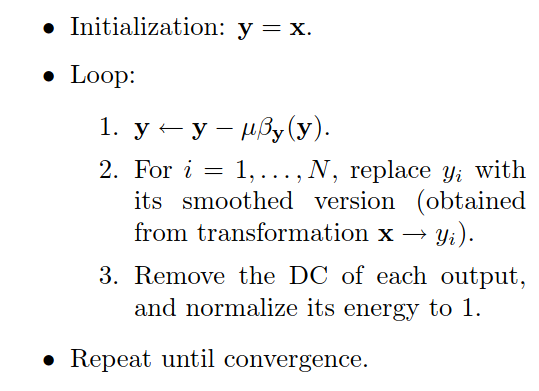
\includegraphics[scale=0.5]{Figures/alg.png}
\end{figure}

این الگوریتم قابل تعمیم به فرآیند‌های تصادفی نیز هست. برای این کار، کافی است در هر مرحله، شیفتی تصادفی از یکی از فرآیند‌های تصادفی در نظر گرفت و الگوریتم فوق را بر روی این ورژن شیفت یافته انجام داد.

\section{شبیه‌سازی عملکرد الگوریتم}
در این شبیه‌سازی، منابع دو فرآیند تصادفی
\lr{ARIMA}
مستقل
با 


\lr{
	\texttt{model = arima('Constant',0.3,'AR',0.7,'MA',0.4,...\\
		'Distribution',tdist,'Variance',0.15)}}


ساخته و با تابع غیرخطی: 
\begin{equation}
\begin{cases}
x_1(t) = s_1(t) + 0.5s_2(t) + 0.5s_1(t)s_2(t)\\
x_2(t) = 0.6s_2(t) + 2s_2(t) + 0.3s_1(t)s_2(t)
\end{cases}
\end{equation}
مخلوط  می‌کنیم. الگوریتم را بر مخلوط‌ها اعمال کرده و مقدار
\lr{SNR}
جداسازی را بر حسب تعداد تکرار الگوریتم رسم می‌کنیم.
\begin{figure}[h!]
	\centering
	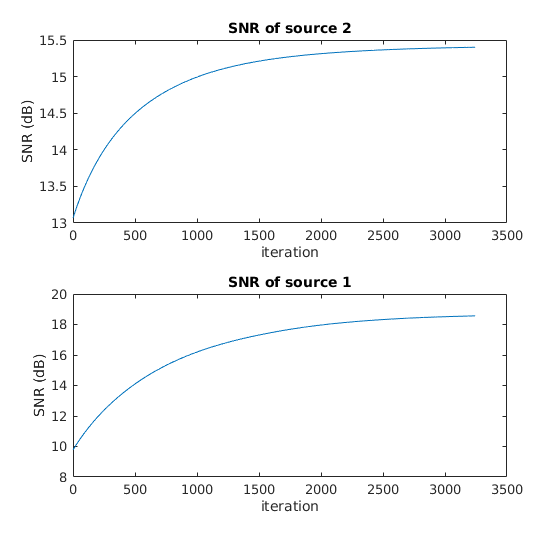
\includegraphics[scale=0.8]{Figures/snr.png}
	\caption{
		\lr{SNR}
		جداسازی مخلوط غیرخطی با کمینه‌کردن اطلاعات متقابل
	}
\end{figure}

این الگوریتم، قادر به رسیدن به 
\lr{SNR}
ای برابر با 
$15.5 dB$
و 
$18.0 dB$
است که عملکردی بسیار قابل قبول است.

\chapter{جداسازی کور  فرآیند‌های گوسی}
\label{chapter:gaussian}
در این فصل به بررسی ایده‌هایی برای جداسازی مخلوط‌های غیرخطی فرآیند‌های تصادفی گوسی می‌پردازیم. همان‌طور که در قضیه‌ی 
\eqref{darmois_skitovic}
دیدیم، جداسازی فرآیند‌های تصادفی و همچنین متغیر‌های تصادفی گوسی، حتی در صورت خطی بودن نیز مسئله‌ای دشوار است. چندین الگوریتم با تضمین‌های تئوری وجود دارند که با بهره‌گیری از روابط زمانی موجود در منابع، به جداسازی کور مخلوط‌های خطی فرآیند‌های گوسی می‌پردازند. نمونه‌هایی از این الگوریتم‌ها را می‌توانید در 
\cite{comon2010handbook}
بیابید.  در این فصل، تمرکز ما بر الگوریتم‌هایی برای تبدیل مخلوط‌های غیرخطی به مخلوط‌های خطی خواهد بود تا در ادامه‌، با بهره‌گیری از الگوریتم‌های جداسازی مخلوط‌های خطی، جداسازی منابع را به صورت کامل انجام دهیم. در این‌جا مخلوط‌ها را آنی در نظر گرفته، یعنی هر سیستم مخلوط‌کننده، به صورت یک تابع
 $\mathbb{R}^n \to  \mathbb{R}^n$
 مدل می‌شود.

\section{ایده‌ی اصلی}
ایده‌ی اصلی تبدیل مخلوط‌های غیرخطی به خطی، این است که تابعی خطی ساز را بیابیم که ویژگی گوسی بودن را فرآیند‌های تصادفی برگرداند. منابع
$\mathbf{s}(t) \in \mathbb{R}^n$
 فرآیند‌های تصادفی گوسی هستند. این منابع، بعد از گذر از تابع مخلوط‌کننده‌ی 
 $\mathbf{f}: \mathbb{R}^n \to  \mathbb{R}^n$
 احتمالاً خاصیت گوسی بودن خود را از دست می دهند و ما تابع 
$\mathbf{g}: \mathbb{R}^n \to  \mathbb{R}^n$
را به نحوی می‌یابیم که
$\g \circ \f (\s)$
مجدداً $n$ فرآیند گوسی شود.  
 
 
 فرض کنید می  دانیم که تابع مخلوط‌کننده‌ی 
 $\f$،
 عضوی از خانواده‌ی توابع 
 $\mathcal{F}$
 است. سیستم جداسازی خود را نیز از مجموعه‌ی توابع 
$\mathcal{G}$
  انتخاب می‌کنیم. حال مجموعه‌ی توابع
 $\mathcal{H} = \{\f \circ \g | \f \in \mathcal{F}, \g \in \mathcal{G}\}$
 را در نظر بگیرید. اگر نشان دهیم که در بین توابع موجود در 
 $\mathcal{H}$،
این  تنها تابع خطی است که خاصیت گوسی بودن را حفظ می‌کند، به هدف خود دست یافته‌ایم. چنین قضیه‌ای به آن معنا است که اگر تابعی جداساز بیابیم که گوسی بودن خروجی را تضمین می‌کند، تضمین‌ کرده‌ایم که خروجی سیستم جداساز، برابر اعمال یک تابع خطی بر ورودی‌هاست: مخلوط خطی‌سازی شده است. 

در ادامه‌ی این فصل، به بررسی مجموعه‌های مختلف توابع پرداخته و این شرط را در آن‌ها مورد بررسی قرار می دهیم.

\section{مخلوط‌های کلّی}
شاید به نظر برسید که تنها تابع پیوسته‌ی که قادر به حفظ خاصیت گوسی بودن است، تابع خطی است. این گزاره در حالت کلی نادرست است و مثال‌های نقض بسیاری برای آن وجود دارد. در این جا به بیان دو مثال نقض اکتفا می‌کنیم.
\begin{example}
فرض کنید 
$F_1$
تابع CDF یک توزیع
$\chi^2(1)$
است و 
$\Phi$
تابع 
CDF
گوسی استاندارد است. در این صورت،
$\Phi^{-1}(F_1(X^2))$
یک تابع غیرخطی، و پیوسته است که گوسی بودن $X$ را حفظ می‌کند.
\end{example}

\begin{example}
 فرض کنید $X$ و $Y$ دو متغیر تصادفی گوسی باشند. در این صورت، تابع 
 
 \begin{equation}
\begin{cases}
Y_1 = \frac{X_1^2 - X_2^2}{\sqrt{X_1^2 + X_2^2}}\\
Y_2 = \frac{2X_1X_2}{\sqrt{X_1^2 + X_2^2}}
\end{cases}
 \end{equation}
 گوسی بودن را حفظ می‌کند.
\end{example}


حال به بررس یک مثال کلّی‌تر می‌پردازیم.
\begin{theorem}
فرض کنید 
$\s \in \mathbb{R}^n$
یک بردار تصادفی گوسی استاندارد باشد. همچنین فرض کنید تابع 
$\h: \mathbb{R}^n \to \mathbb{R}^n$
یک تابع مشتق‌پذیر با مشتق پیوسته و یک به یک است. اگر $\h$ شرایط زیر را ارضا کند،
$\h(\s)$
گوسی است:
\begin{itemize}
\item 
تابع 
$\h$
حفظ ‌کننده‌ی نرم است.

\item 
دترمینان ماتریس ژاکوبی $\h$ برابر یک است، یعنی
$\forall \s: \; |J_\h(\s)| = 1$.
\end{itemize}

به این دسته از توابع، دوران‌ تعمیم‌یافته می گوییم.
\end{theorem}

\begin{proof}
از احتمال مقدماتی به یاد داریم که اگر 
$\h$
مشتق‌پذیر باشد، آنگاه
\begin{equation}
\y = \h(\s) \implies p_\Y(\y) = \frac{p_{\mathbf{S}}(\s)}{|J_\h(\s)|}.
\end{equation}

با جای‌گذاری تابع چگالی احتمال بردار استاندارد گوسی، داریم:
\begin{equation}
p_{\mathbf{Y}}(\y) = \frac{1}{|J_\h(\s)|}\frac{1}{\sqrt{2\pi^n}}\exp(-\frac{1}{2} \s^T\s) = \frac{1}{\sqrt{2\pi^n}} \exp(-\frac{1}{2} \y^T \y) 
\end{equation}
که تساوی دوم، از دو شرط قضیه به دست آمده است.

\end{proof}

\begin{remark}
با توجه به اثبات قضیه‌ی فوق، به سادگی می‌توان دید که اگر 
$\s$
برداری گوسی با درایه‌های مستقل بوده و
$\h$
یک دوران تعمیم یافته باشد،
$\h(\s)$
 نیز یک بردار گوسی با درایه‌های مستقل است.
\end{remark}
\section{مخلوط‌های چندجمله‌ای}

در این فصل، به بررسی خواص توابع چندجمله‌ای می‌پردازیم. یک چند‌جمله‌ای بعد بالا را بدین صورت تعریف می‌کنیم.
\begin{definition}
تابع 
$\f: \mathbb{R}^n \to \mathbb{R}^n$
و 
$\f(\x) = \Big(f_1(\x), f_2(\x), \dots, f_n(\x)\Big)^T$
را یک چندجمله‌ای بعد بالا می‌گوییم اگر تمام توابع 
$f_i$
چندجمله‌ای باشند.
\end{definition}

حال اثبات می‌کنیم که تنها توابع چند‌جمله‌ای خطی می‌توانند گوسی بودن را حفظ کنند.

\begin{theorem}
	فرض کنید $n$متغیر تصادفی 
	$s_1, s_2, \dots, s_n$
	متغیرهای تصادفی مشترکاً گوسی باشند و 
	$\mathbf{p}: \mathbb{R}^n\to\mathbb{R}^n$
	نیز یک نگاشت چند‌جمله‌ای دلخواه باشد و داشته باشیم
	$\mathbf{y} = \mathbf{p}(\mathbf{s}) $.
	متغیرهای تصادفی 
	$y_1, y_2, \dots, y_n$،
	مشترکاً گوسی هستند اگر و تنها اگر
	$$\mathbf{p}(\mathbf{s}) = \mathbf{A}\mathbf{s} + \mathbf{b}$$
	که در آن 
	$\mathbf{A} \in \mathbb{R}^{n\times n}$
	و 
	$\mathbf{b} \in \mathbb{R}^n$
	هستند.
\end{theorem}

\begin{proof}
میانگین 
$\s$
و 
$\y$
را  به ترتیب
$\mu_\s$
و 
$\mu_\y$
و ماتریس کوواریانس آنها را به ترتیب
$\bf K_\s$
و
$\bf K_\y$
بگیرید. تابع چگالی احتمال بردارهای تصادفی 
$\s$
و 
$\y$
برابر است با

\begin{align}
\label{E_NormalPDF1}
p_S({\bf s}) &= \frac{1}{\sqrt{(2\pi)^n|{\bf K}_{\bf s}|}} \ e^{\frac{-1}{2}({\bf s}-\boldsymbol{\mu}_{\bf s})^\top{\bf K}_{\bf s}^{-1}({\bf s}-\boldsymbol{\mu}_{\bf s})} \\
\label{E_NormalPDF2}
p_Y({\bf y}) &= \frac{1}{\sqrt{(2\pi)^n|{\bf K}_{\bf y}|}} \ e^{\frac{-1}{2}({\bf y}-\boldsymbol{\mu}_{\bf y})^\top{\bf K}_{\bf y}^{-1}({\bf y}-\boldsymbol{\mu}_{\bf y})}.
\end{align}

با توجه به پیوسته بودن توابع، می‌توان تابع چگالی احتمال 
$\s$
و 
$\y$
 را با رابطه‌ی زیر به هم ربط داد:
 \begin{equation}
 \label{E_PolynomialPDF}
 p_Y({\bf y})=\frac{p_S({\bf s})}{|{\bf J}_{\bf p}|}
 \end{equation}
 که در آن
 ${\bf J}_{\bf p}$
 ماتریس ژاکوبی تبدیل $\bf p$ است. از آن‌جایی که تمام المان‌های ماتریس ژاکوبی یک چندجمله‌ای، چندجمله ای هستند، دترمینان آن نیز به صورت قدر مطلق یک چند جمله‌ای نوشته می‌شود، یعنی
 $|{\bf J}_{\bf p}| = |q(\s)|$.

بنابراین، با توجه به معادله‌ی 
 \eqref{E_PolynomialPDF}
 داریم
 $$|q(\s)| p_Y(\y) = p_S(\s) \implies \ln |q(\s)| + \ln p_Y(\y) = \ln p_S(\s)$$
 با جای‌گذاری 
 \eqref{E_NormalPDF1}
 داریم
 \begin{multline}
 \ln |q({\bf s})| - \frac{1}{2} \ln |{\bf K}_{\bf y}|
 - \frac{1}{2} ({\bf y}-\boldsymbol{\mu}_{\bf y})^\top{\bf K}_{\bf y}^{-1}({\bf y}-\boldsymbol{\mu}_{\bf y}) = \\ - \frac{1}{2} \ln |{\bf K}_{\bf s}|
 - \frac{1}{2} ({\bf s}-\boldsymbol{\mu}_{\bf s})^\top{\bf K}_{\bf s}^{-1}({\bf s}-\boldsymbol{\mu}_{\bf s}),
 \end{multline}
 یه به صورت معادل
 \begin{equation}
 \label{E_MainEQMainTheorem}
 c + ({\bf y}-\boldsymbol{\mu}_{\bf y})^\top{\bf K}_{\bf y}^{-1}({\bf y}-\boldsymbol{\mu}_{\bf y}) =
 ({\bf s}-\boldsymbol{\mu}_{\bf s})^\top{\bf K}_{\bf s}^{-1}({\bf s}-\boldsymbol{\mu}_{\bf s}) + 2\ln |q({\bf s})|
 \end{equation}
 که در آن
 $c =  \ln (|{\bf K}_{\bf y}|/|{\bf K}_{\bf s}|)=\ln |{\bf K}_{\bf y}{\bf K}_{\bf s}^{-1}|$.


معادله‌ی 
 \eqref{E_MainEQMainTheorem}
 برای هر 
 $\s$
 برقرار است. آن را در 
 $\s = (s, s, \dots, s)^T$
که
$s\in \mathbb{R}$
 محاسبه می‌کنیم.  تعریف می‌کنیم
 ${\bf p}(\s) = \tilde{{\bf p}}(s)$
 و 
 $\tilde{{q}}(\s) = q(s)$.
 به عبارت دیگر
 \begin{equation}
 {\bf s}=s\boldsymbol{1}_{n \times 1} \Rightarrow
 {\bf y}=\tilde{\bf p}(s)=[\ \tilde{p}_1(s),\dots,\tilde{p}_n(s)\ ]^\top
 \end{equation}
 
ضرایب چندجمله‌ ای‌ها را به صورت زیر نمایش می‌دهیم:
 \begin{align}
 \label{E_ParticularCase1}
 \forall 1 \le k \le n \quad
 \tilde{p}_k(s) &= \sum_{j=0}^{d_k} a_{kj}s^{j} \\
 \label{E_ParticularCase2}
 \tilde{q}(s) &= \sum_{i=0}^{d_{\bf J}} b_{i}s^{i}.
 \end{align}
با جای‌گذاری
\eqref{E_ParticularCase1} و
\eqref{E_ParticularCase2} 
در
\eqref{E_MainEQMainTheorem} 
داریم
\begin{align}
\label{E_ParticularMainEQ}
c + (\tilde{\bf p}(s)-\boldsymbol{\mu}_{\bf y})^\top
&
{\bf K}_{\bf y}^{-1}(\tilde{\bf p}(s)-\boldsymbol{\mu}_{\bf y}) \nonumber \\
&= (s \boldsymbol{1}_{n \times 1}-\boldsymbol{\mu}_{\bf s})^\top{\bf K}_{\bf s}^{-1}(s \boldsymbol{1}_{n \times 1}-\boldsymbol{\mu}_{\bf s}) + 2\ln |\tilde{q}(s)| \nonumber \\
&= \alpha s^2 + \beta s + \gamma + 2\ln |\tilde{q}(s)|.
\end{align}
که در آن
$\alpha = \boldsymbol{1}_{n \times 1}^\top{\bf K}_{\bf s}^{-1}\boldsymbol{1}_{n \times 1}$, $\beta = -2\boldsymbol{1}_{n \times 1}^\top{\bf K}_{\bf s}^{-1}\boldsymbol{\mu}_{\bf s}$ 
و
 $\gamma = \boldsymbol{\mu}_{\bf s}^\top{\bf K}_{\bf s}^{-1}\boldsymbol{\mu}_{\bf s}$.
 در 
$s$
های بزرگ، سمت راست این معادله به صورت یک تابع درجه دوم عمل می‌کند، در نتیجه 
$\tilde{\bf p}(s)$
و 
${\bf p}(\s)$
شامل جملاتی با درجه‌ی حداکثر یک هستند. یعنی چندجمله‌ای خطی است.

\end{proof}
با توجه به این قضیه‌، می‌توان به  نتیجه‌ی کاربردی زیر رسید.

\begin{corollary}
	\label{corrr}
	فرض کنید 
	$\mathbf{s}(t) = [s_1(t), s_2(t), \dots, s_n(t)]^\top$
	و
	$\mathbf{x}(t)= [x_1(t), x_2(t), \dots, x_n(t)]^\top$
	دو بردار تصادفی $n$ بعدی منابع و مشاهدات بوده و هر یک از
	$s_i(t)$
	ها نیز یک فرآیند تصادفی گوسی باشد. منابع با تابع
	$$\mathbf{x}(t) = \mathbf{f}(\mathbf{s}(t))$$
	مخلوط‌شده‌اند که در آن
	$\mathbf{f}$
	یک تابع مجهول چندجمله‌ای است. اگر چندجمله‌ای 
	$\mathbf{g}$
	پیدا شود به نحوی که 
	$\mathbf{y}(t) = \mathbf{g}(\mathbf{x}(t))$
	نیز برداری از $n$ فرآیند تصافی گوسی باشد، آنگاه 
	$\mathbf{h} = \mathbf{g}\circ \mathbf{f} $
	تابعی خطی است.
\end{corollary}



\section{معرفی الگوریتم‌های مختلف جداسازی}
به کمک نتیجه‌ی
\eqref{corrr}،
 می‌توان الگوریتمی برای خطی‌سازی مخلوط‌های غیرخطی ارائه داد. این الگوریتم، مدلی پارامتری برای چندجمله‌ای جداسازی در نظر گرفته و پارامترهای آن را به نحوی مشخص می‌کند که معیاری از گوسی بودن متغیر‌های خروجی بیشینه شود. در مدل زیر، ماتریس 
$\boldsymbol{\Theta}$
ماتریس ضرایب چند‌جمله‌ای جداسازی است و 
$\mathbf{k}$
بردار تک‌جمله‌ای ها از درجه‌ی مطلوب است.

\begin{equation*}
\label{E_Parametrizing}
{\g}({\x})=
\begin{bmatrix}
g_1({\x}) \\
g_2({\x}) \\
\vdots \\
g_n({\x})
\end{bmatrix}=
\begin{bmatrix}
\boldsymbol{\theta_1}^\top \\
\boldsymbol{\theta_2}^\top\\
\vdots \\
\boldsymbol{\theta_n}^\top
\end{bmatrix}{\mathbf{k}}({\x})=
\boldsymbol{\Theta}{\mathbf{k}}({\x})
\end{equation*}

معیارهای بسیار مختلفی از گوسی بودن وجود دارند، آنتروپی‌منفی و کومولان‌های مرتبه‌ی چهارم مثال‌هایی از این معیار‌ها هستند. فرض کنید 
$\mathcal{J}(\mathbf{X})$
معیار از گوسی بودن بردار تصادفی 
$\mathcal{J}(\mathbf{X})$
باشد که به کمک نمونه‌هایی از این بردار تخمین‌زده شده‌است. الگوریتم جداسازی مناسب، 
\begin{equation*}
\underset{\boldsymbol{\Theta}}{\min} \ \| \boldsymbol{\mathcal{J}}(\boldsymbol{\Theta}{\mathbf{k}}({\x})) \|_2^2
\end{equation*}
است. 

در ادامه، سه معیار مختلف گوسی بودن را مورد بررسی قرار می‌دهیم. 



\subsection{آنتروپی منفی}
از نظریه‌ی اطلاعات کلاسیک می‌دانیم که در بین توزیع‌های احتمال با واریانس یک‌سان، توزیع گوسی دارای بیشترین آنتروپی است
\cite{cover}. 
از این قضیه‌ می توان برای طراحی یک معیار گوسی بودن بهره برد. آنتروپی منفی را برای متغیر تصادفی  $X$ بدین صورت تعریف می‌کنیم

$$\mathcal{J}_1(X) \triangleq  {\bf H}(\tilde{X}) - {\bf H}(X)$$
که ${\bf H}$ نمایش دهنده‌ی آنتروپی و 
$\tilde{X}$
متغیری تصادفی گوسی با واریانسی برابر با واریانس $X$ است.
\subsection{فاصله‌ی کلموگروف}
 نمونه‌های مستقل 
 $X_1, X_2, \dots, X_n$
با توزیع یکسان در اختیار هستند. یک تخمین‌گر ناسوییده برای تابع توزیع تجمعی، برابر است با
$$\hat{F}_n(t) = \frac{1}{n} \sum_{i = 1}^{n} 1_{(-\infty, t)}[X_i]$$
که در آن
$1_{(-\infty, t)}$
تابع مشخص‌کننده‌ی\LTRfootnote{Indicator Function}
رویداد
$\{x\leq t\}$
است. شکل
\eqref{fig:CDF}
 نمونه‌ای از این تابع تخمین‌زده شده را نمایش می‌دهد.
 \begin{figure}[h!]
\centering
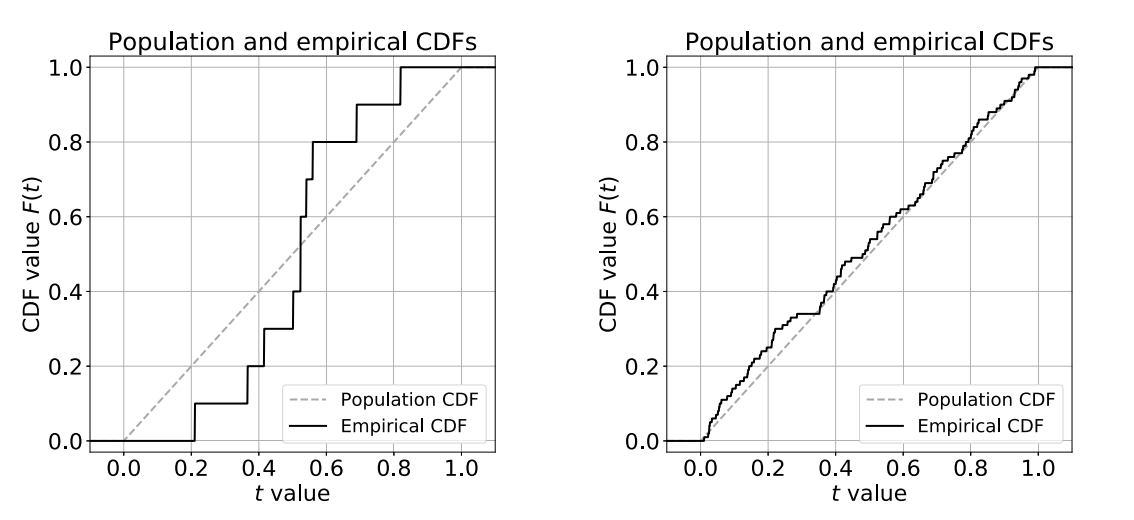
\includegraphics[scale=0.3]{Figures/CDF.png}
\caption{CDF 
تخمين ‌زده‌شده و CDF واقعی برای توزیع یکنواخت در بازه‌ی 
$[0, 1]$.
}
\label{fig:CDF}
 \end{figure}
 
قضیه‌ی کلاسیک
\lr{Glivenko-Cantelli}
همگرایی یکنواخت (به ازای تمام $t$ ها) های تابع 
CDF
تجربی به تابع  
CDF
واقعی را بیان می‌کند.

\begin{theorem}
برای هر توزیع دلخواه، با احتمال یک داریم
$$||\hat{F}_n - F||_\infty \to 0$$
\end{theorem}
\begin{proof}
این نتیجه، یکی از نتایج ابتدایی آمار بعد بالا است. به عنوان مثال، فصل چهارم کتاب 
\cite{wainwright_2019}
ببینید.
\end{proof}

معیار زیر را به عنوان یک فاصله از توزیع گوسی تعریف می‌کنیم.

$$\mathcal{J}_2(X) = \sup_x|F_X(x) - \Phi(x)|$$
که در آن 
$\phi(x)$
تابع CDF متغیر تصادفی گوسی، با واریانس برابر با $X$ است. می‌توان این کمیت‌را به صورت زیر تخمین زد
$$\hat{\mathcal{J}}_2(X) = \sup_x|\hat{F}_X(x) - \Phi(x)|.$$

این معیار گوسی بودن را فاصله‌ی کولموگروف می‌نامیم.
\begin{corollary}
از قضیه‌ی فوق نتیجه می‌شود که در صورت گوسی بودن متغیر تصادفی $X$، تخمین‌گر
$\hat{\mathcal{J}}_2(X)$
با احتمال یک به صفر میل می‌کند. همچنین در صورت گوسی نبودن، این تخمین‌گر به عددی مثبت میل می‌کند.
\end{corollary}
\subsection{کرتسیس}
معیار گوسی بودن مبتنی بر کرتسیس یه متغیر تصادفی
$X$
را به صورت زیر تعریف می‌کنیم
$$\mathcal{J}_3(X) =  \Big[\mathbb{E}[X^4] - 3\big(\mathbb{E}[X^2]\big)^2\Big]^2.$$

از احتمال مقدماتی می‌دانیم که این معیار، برای متغیر‌های تصادفی گوسی صفر، و برای مابقی متغیرهای تصادفی مثبت است.


\section{مقایسه‌ی الگوریتم‌های مختلف}
  تابع مخلوط‌کننده‌ی 
\begin{equation*}
\f\Big([s_1, s_2]^T\Big) = [s_1 + (s_1+s_2)^3, s_2 - (s_1+s_2)^3]^T
\end{equation*}
را در نظر بگیرید. این یک چندجمله‌ای وارون‌پذیر، با وارون چندجمله‌ای است. وارون این تابع برابر است با
\begin{equation*}
\g\Big([x_1, x_2]^T\Big) = [x_1 - (x_1+x_2)^3, x_2 - (x_1+x_2)^3]^T
\end{equation*}
برای مقایسه‌ روش‌های مختلف، از این مخلوط استفاده می‌کنیم. مدل پارامتری را یک چندجمله‌ای درجه سوم با ۱۰ ضریب می‌گیریم. 
در شکل
\eqref{fig:comp}،
با ثابت نگه‌داشتم هشت ضریب در نقطه‌ی بهینه، و تغییر دو ضریب، تابع هزینه‌ی الگوریتم‌های مختلف را رسم کرده‌ایم.


\begin{figure}[h!]
\centering
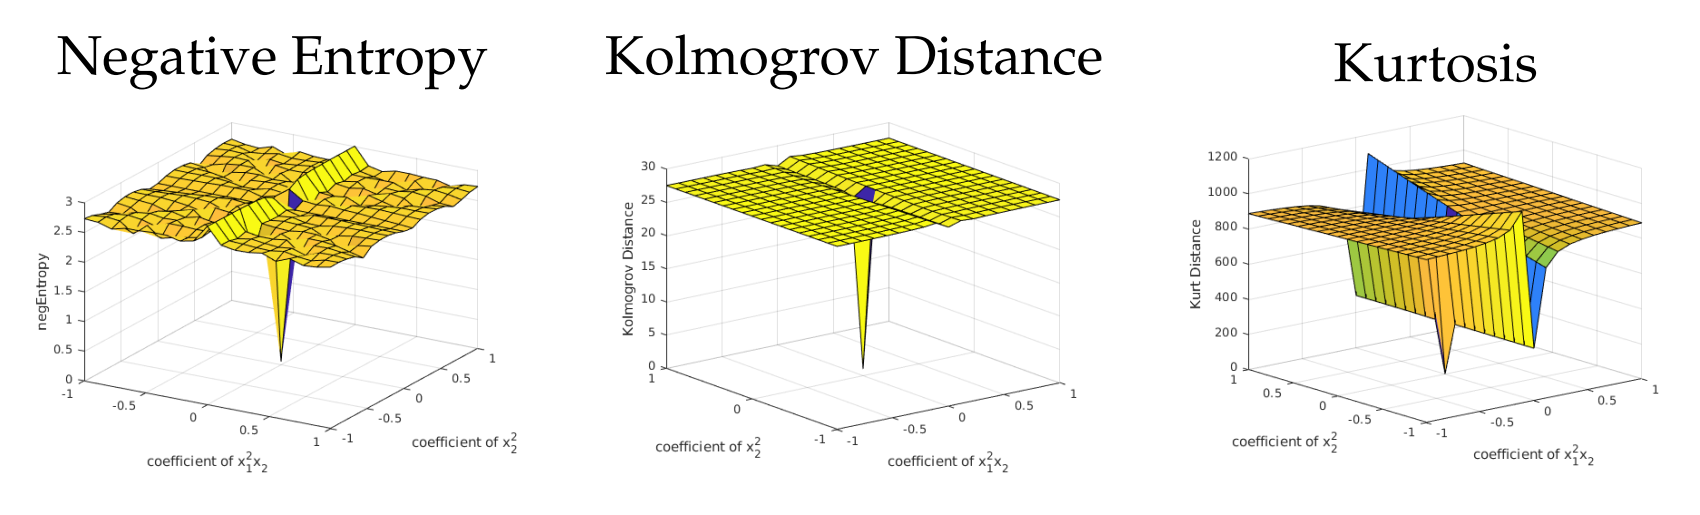
\includegraphics[scale=0.25]{Figures/comp.png}
\caption{مقدار تابع هزینه‌ی الکوریتم بهینه‌سازی حول نقطه‌ی بهینه. دو بعد تغییر داده‌شده‌اند و مابقی ابعاد بر روی مقدار بهینه ثابت مانده‌اند.}
\label{fig:comp}
\end{figure}

دیده‌می‌شود که هر سه الگوریتم، در نقطه‌ی بهینه مقدار بسیار کوچک‌تری به نسبت سایر نقاط را اخذ می‌کنند. الگوریتم مبتنی با فاصله‌ی کلموگروف نیز تابع هزینه‌ی هموارتری به نسبت الگوریتم مبتنی بر آنتروپی منفی دارد. در ادامه، برای هر الگوریتم ده نمودار رسم خواهیم کرد که بیان‌گر تغییرات مقدار تابع هزینه‌ی آن الگوریتم، با تغییر یکی از ضرایب و ثابت نگه‌داشتم مابقی ضرایب در نقطه‌ی بهینه‌ی آن‌ها است.

\newpage

\begin{figure}[h!]
	\centering
	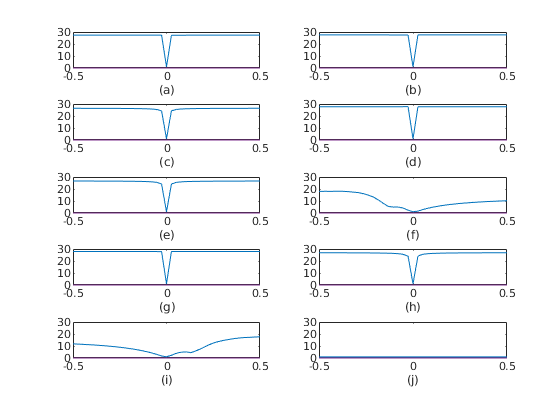
\includegraphics[scale=0.75]{Figures/kolmo1.png}
	\caption{
		تغییرات مقدار تابع هزینه‌ی الگوریتم مبتنی با فاصله‌ی کلموگروف، با تغییر یکی از ضرایب و ثابت نگه‌داشتم مابقی ضرایب در نقطه‌ی بهینه‌ی آن‌ها.
	}
	\label{fig:comp1}
\end{figure}
\begin{figure}[h!]
	\centering
	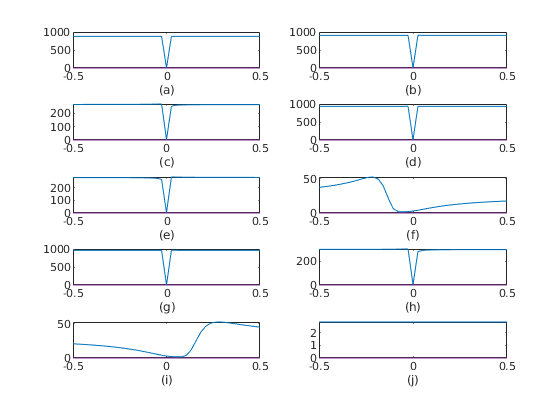
\includegraphics[scale=0.7]{Figures/kurt1.png}
		\caption{
		تغییرات مقدار تابع هزینه‌ی الگوریتم مبتنی با فاصله‌ی کرتسیس، با تغییر یکی از ضرایب و ثابت نگه‌داشتم مابقی ضرایب در نقطه‌ی بهینه‌ی آن‌ها.
	}
	\label{fig:comp2}
\end{figure}

\newpage
\begin{figure}[h!]
	\centering
	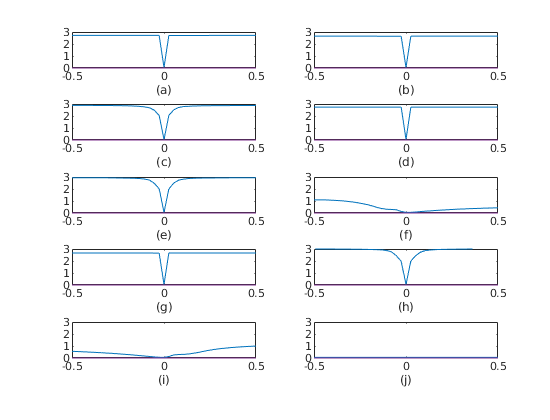
\includegraphics[scale=0.75]{Figures/negent1.png}
	\caption{
		تغییرات مقدار تابع هزینه‌ی الگوریتم مبتنی با فاصله‌ی آنتروپی منفی، با تغییر یکی از ضرایب و ثابت نگه‌داشتم مابقی ضرایب در نقطه‌ی بهینه‌ی آن‌ها.
	}
	\label{fig:comp3}
\end{figure}

\chapter{جمع‌بندی}

در این پروژه، به بررسی نتایج تئوری و تلاش‌های موجود برای اثبات قضیه‌ی جدایی‌پذیری مخلوط‌های غیرخطی فرآیند‌های تصادفی خطی و غیرخطی پرداختیم. نشان دادیم که در حالت کلّی، جداسازی مخلوط‌های غیرخطی غیرممکن است و مثال‌هایی از مسائل غیرخطی معرفی کردیم که در آن‌ها مخلوط‌های غیرخطی جدایی‌پذیر نیستند. بعد از مرور الگوریتم‌های کمینه‌سازی اطلاعات متقابل و کاربرد‌های آن‌ها در جداسازی مخلوط‌های خطی، الگوریتمی مشابه برای جداسازی مخلوط‌های غیرخطی ارائه و عملکرد تجربی این الگوریتم را بررسی نمودیم. در انتها به مطالعه‌ی مخلوط‌های غیرخطی فرآیند‌های تصادفی گوسی و ارائه‌ی الگوریتم‌هایی برای جداسازی این مخلوط‌ها پرداختیم و الگوریتم‌ها را نیز از نظر کارکرد با یکدیگر مقایسه کردیم.
\bibliography{bib, long}
\bibliographystyle{ieeetr-fa}

\PrepareForLatinPages
\date{Summer 2020}
\title{\sffamily Blind Separation of Nonlinear Mixtures of Stochastic Processes}
\author{\sffamily Behrad Moniri}
\university{Sharif University of Technology\\Department of Electrical Engineering}
\subject{Electrical Engineering}
\supervisor{\sffamily Prof. Massoud Babaie-Zadeh}
\consult{\sffamily Prof. Mohammad Memarian}

\makethesistitle
\end{document}